\documentclass[11pt,a4paper,final]{article} 
\usepackage[english, russian]{babel}
\usepackage[final]{pdfpages}
\usepackage{textcomp,enumitem}
\usepackage{amsmath,amssymb,cmap,pgfplots,pgfplotstable}
\usepackage{pdflscape}
\usepackage{eso-pic}
\usepackage{graphics}
%\usepackage{fancyhdr}
\usepackage{rotating}
\usepackage{upgreek}
\usepackage{tipa}
\usepackage{tikz}
\usepackage{amsfonts}
\usepackage{caption}
\usepackage{subcaption}
\usepackage{float}
\usepackage{pgfplots}
\usepackage{indentfirst}
\usepackage[T2A]{fontenc}
\usepackage[utf8]{inputenc} 
\usepackage[left=2cm,right=2cm,top=2cm,bottom=3cm,bindingo ffset=0cm, 
]{geometry}
\usepackage{longtable}
\usepackage{array}
\usepackage{multirow}
\usepackage{setspace}
\usepackage[unicode, pdftex, colorlinks, urlcolor=blue]{hyperref}
\usepackage{listings} % Для красивого оформления кода
\usepackage{xcolor}
\usepackage{cmap}
\usepackage{amsmath}
\usepackage{mathabx}
\usepackage{graphicx} % Для \rotatebox
%\usepackage{layouts}
\usepackage{calc}




\usetikzlibrary{arrows,calc,intersections}
\addto\captionsrussian{\def\refname{}}
\pgfplotsset{compat=newest}
\pgfplotsset{compat=1.9}
\onehalfspacing
\pagestyle{plain}



\lstdefinestyle{sqlstyle}{
    language=SQL,
    basicstyle=\ttfamily\small,
    keywordstyle=\color{blue}\bfseries,
    commentstyle=\color{green!50!black}\itshape,
    stringstyle=\color{red},
    numbers=left,
    numberstyle=\tiny\color{gray},
    stepnumber=1,
    numbersep=5pt,
    backgroundcolor=\color{white},
    frame=single,
    rulecolor=\color{black},
    breaklines=true,
    breakatwhitespace=true,
    tabsize=4,
    showstringspaces=false,
    inputencoding=utf8,
    extendedchars=true,
    literate=
    {а}{{\selectfont\char224}}1
    {б}{{\selectfont\char225}}1
    {в}{{\selectfont\char226}}1
    {г}{{\selectfont\char227}}1
    {д}{{\selectfont\char228}}1
    {е}{{\selectfont\char229}}1
    {ё}{{\selectfont\char184}}1
    {ж}{{\selectfont\char230}}1
    {з}{{\selectfont\char231}}1
    {и}{{\selectfont\char232}}1
    {й}{{\selectfont\char233}}1
    {к}{{\selectfont\char234}}1
    {л}{{\selectfont\char235}}1
    {м}{{\selectfont\char236}}1
    {н}{{\selectfont\char237}}1
    {о}{{\selectfont\char238}}1
    {п}{{\selectfont\char239}}1
    {р}{{\selectfont\char240}}1
    {с}{{\selectfont\char241}}1
    {т}{{\selectfont\char242}}1
    {у}{{\selectfont\char243}}1
    {ф}{{\selectfont\char244}}1
    {х}{{\selectfont\char245}}1
    {ц}{{\selectfont\char246}}1
    {ч}{{\selectfont\char247}}1
    {ш}{{\selectfont\char248}}1
    {щ}{{\selectfont\char249}}1
    {ъ}{{\selectfont\char250}}1
    {ы}{{\selectfont\char251}}1
    {ь}{{\selectfont\char252}}1
    {э}{{\selectfont\char253}}1
    {ю}{{\selectfont\char254}}1
    {я}{{\selectfont\char255}}1
    {А}{{\selectfont\char192}}1
    {Б}{{\selectfont\char193}}1
    {В}{{\selectfont\char194}}1
    {Г}{{\selectfont\char195}}1
    {Д}{{\selectfont\char196}}1
    {Е}{{\selectfont\char197}}1
    {Ё}{{\selectfont\char168}}1
    {Ж}{{\selectfont\char198}}1
    {З}{{\selectfont\char199}}1
    {И}{{\selectfont\char200}}1
    {Й}{{\selectfont\char201}}1
    {К}{{\selectfont\char202}}1
    {Л}{{\selectfont\char203}}1
    {М}{{\selectfont\char204}}1
    {Н}{{\selectfont\char205}}1
    {О}{{\selectfont\char206}}1
    {П}{{\selectfont\char207}}1
    {Р}{{\selectfont\char208}}1
    {С}{{\selectfont\char209}}1
    {Т}{{\selectfont\char210}}1
    {У}{{\selectfont\char211}}1
    {Ф}{{\selectfont\char212}}1
    {Х}{{\selectfont\char213}}1
    {Ц}{{\selectfont\char214}}1
    {Ч}{{\selectfont\char215}}1
    {Ш}{{\selectfont\char216}}1
    {Щ}{{\selectfont\char217}}1
    {Ъ}{{\selectfont\char218}}1
    {Ы}{{\selectfont\char219}}1
    {Ь}{{\selectfont\char220}}1
    {Э}{{\selectfont\char221}}1
    {Ю}{{\selectfont\char222}}1
    {Я}{{\selectfont\char223}}1
}

\begin{document}
\newpage
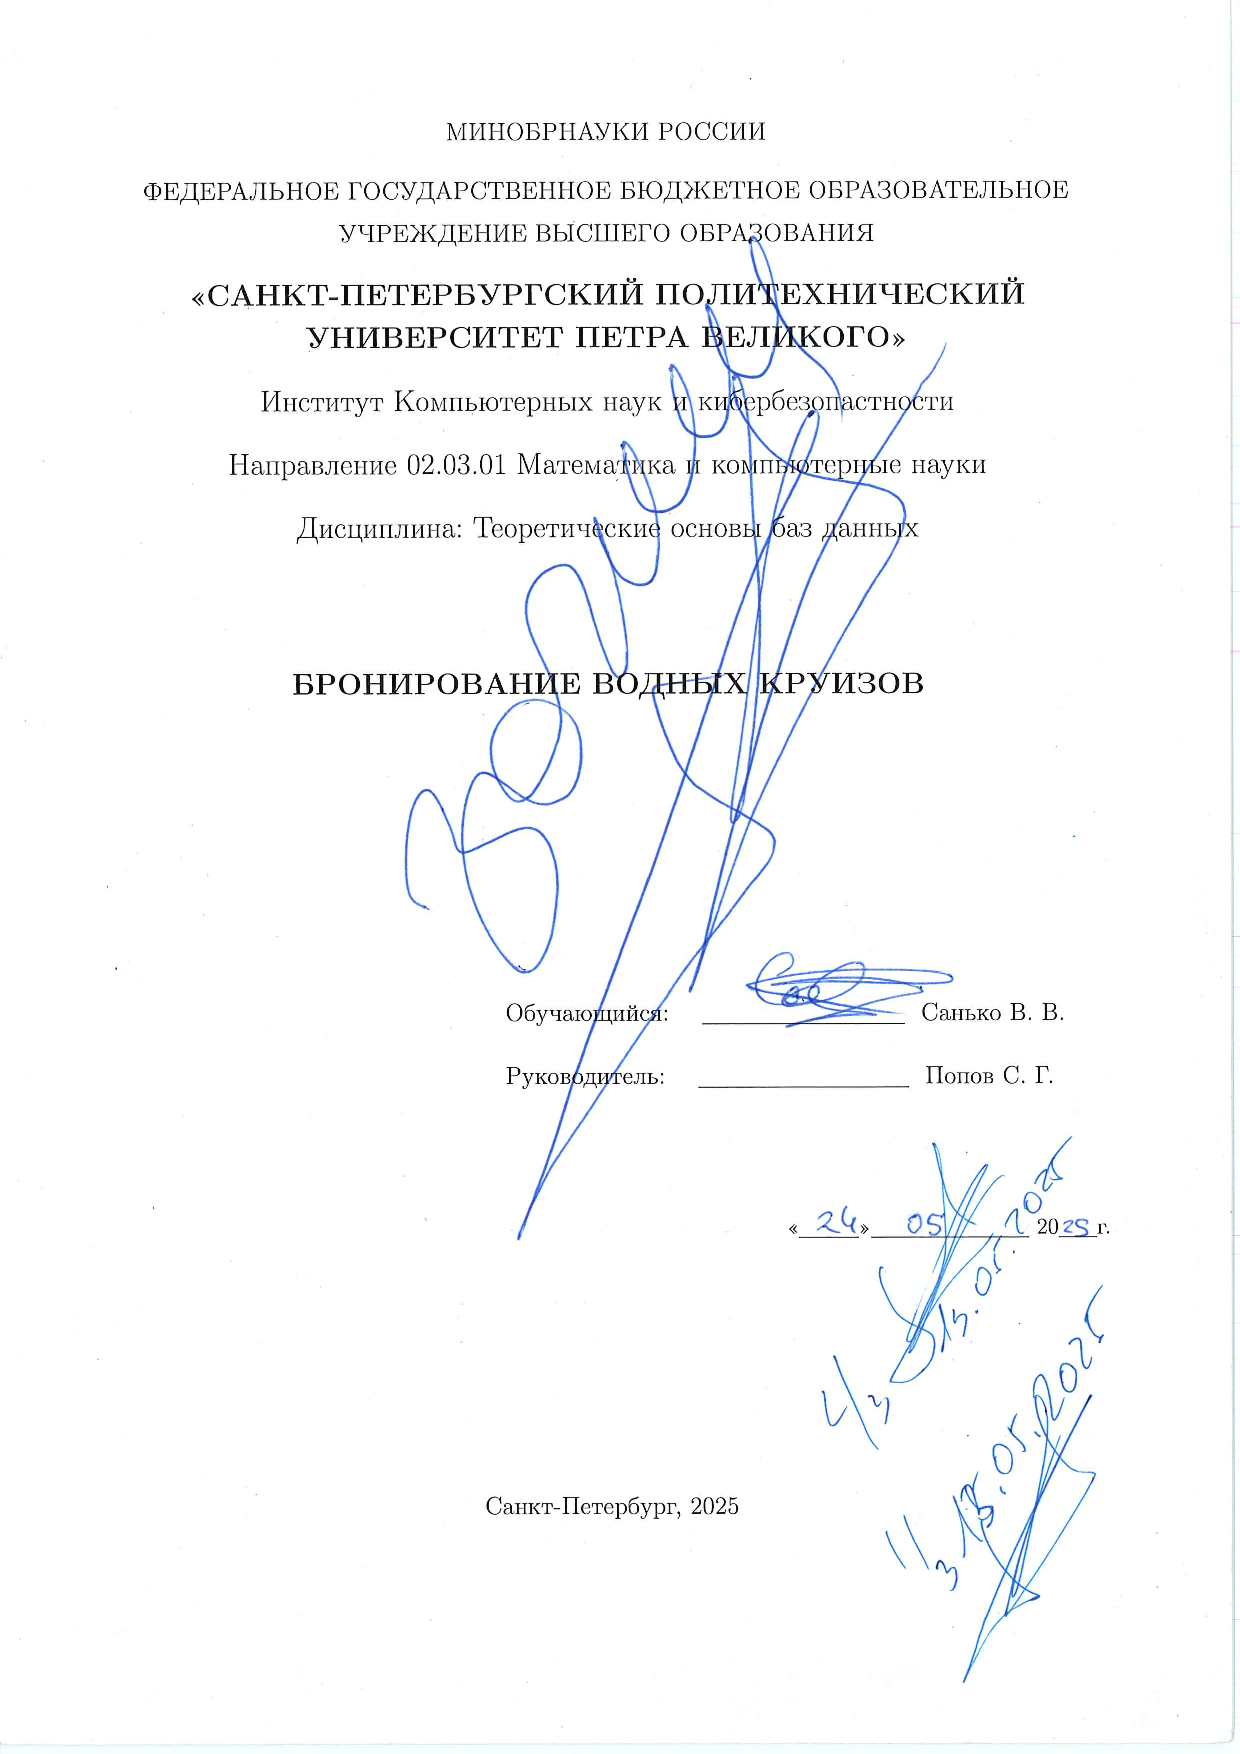
\includepdf[pages={1}, fitpaper=true]{111.pdf}  % Вставляет только 1-ю страницу
\clearpage

\newpage
\section* {Реферат}
\addcontentsline{toc}{section}{Реферат}
Предметной областью данной работы является автоматизация процесса бронирования водных круизов, которая включает в себя управление информацией о клиентах, судах, каютах, круизах и туристических компаниях. Основной задачей является эффективное организация и доступ большим взаимосвязанного данных, используемых для оперативного бронирования и анализа туристической деятельности. Разработанная система может использоваться туристическими фирмами, туроператорами и агентствами для учета круизов, управления клиентской базой, следования допустимости кают и анализа продаж, что дает возможность повысить эффективность и качество обслуживания в водном туризме.

\newpage
\tableofcontents

\newpage
\section* {Введение}
\addcontentsline{toc}{section}{Введение}
В ходе работы была создана база данных, на которой были отображены ключевые сущности, а также связи между ними. Для управления и создания базы данных была определена система управления базами данных MySQL. Создание осуществляется при помощи программы. Также база данных была заполнена в соответсвии с заданием. Для реализации этих этапов использовался язык программирования Python версии 3.8 с библиотекой mysql-connector-python и общими SQL-запросами.

\newpage
\section* {Постановка задачи}
\par Цель работы: реализация функционирующей реляционной базы данных
для салона маникюра и реализация выданных запросов.
\par Задачи работы.
\begin{itemize}
\item Проанализировать предметную область.
\item Создать ER-диаграмму в нотации Чена.
\item Определить цели функционирования базы данных.
\item Спроектировать схему базы данных.
\item Перенести базу данных в «MySQL».
\item Написать текст программы заполнения базы данных.
\item Реализация запросов.
\item Графическое представление результатов запросов.

\end{itemize}


\newpage
\section {Аналитика}
\subsection{Бронирование водного круиза}

 {\par В настоящий момент заказ круиза одна из самых развитых сфер в категории отдыха. Круиз — это форма туризма, представляющая собой путешествие на специально оборудованных судах по водным артериям. Водный круиз, как правило, представляет собой путешествие из одной точки в другую, с дополнительным развлечением на протяжении всего маршрута. В зависимости от маршрута и продолжительности путешествия теплоход делает определенное количество остановок в портовых городах, где пассажиры могут сойти на берег и погулять. По своему типу круизы подразделяются на экскурсионные и туристические, морские и речные, а также длительные и краткосрочные. (Общую информацию о бронировании круизов можно найти на популярных ресурсах, таких как Cruise.com \cite{Cruise.com}). 
 
 Бронирование круиза начинается с выбора туристической компании. Royal Caribbean International – это линия-рекордсмен \cite{Royal}. На сегодняшний день компания является владельцем двух самых больших лайнеров в мире Allure of the Seas и Harmony of the Seas. RCI не строит корабли – она создает плавучие мегаполисы с районами, парками и небоскрёбами. На борту многих кораблей можно встретить собственный аквапарк. Одни из самых крупнейших достижений: Central Park (на Oasis-классе) – первый в мире живой парк на море с 12 000 растений, кафе и вечерними концертами под открытым небом, Neighborhoods (на Icon of the Seas) – 8 тематических зон и Thrill Island (аквапарк с 6 водными горками), The Pearl (на Icon) – гигантская светящаяся сфера-арт-объект, служащая ещё и структурной опорой, Ultimate Abyss – самая высокая горка на море (10 палуб, 14-секундный спуск в темноте), North Star (на Quantum-классе) – стеклянная капсула на высоте 90 метров над водой, Sky Pad – батут с дополненной реальностью.
 
 В России более 30 турфирм, занимающихся организацией водных круизов, самой крупной компанией является ВодоходЪ \cite{vodohod}, на 2018 год охватывавшая 80 $\%$ пассажиропотока. Турфирма - организация, имеющая разрешение на продажу туристических услуг. Турфирма может быть туроператором, а может работать по принципу турагентства. Или даже совмещать оба этих варианта, что нередко случается. Туроператор - это турфирма или лицо (группа людей), которые непосредственно проводят тур, т.е. организовывают снаряжение, питание, инструкторов и разрабатывают маршрут. Турагентство - турфирма, которая помогает туроператору продавать его туры и получает за это комиссионное вознаграждение. Турагентств намного больше, чем туроператоров.
 
 Бронирование круиза начинается с выбора маршрута, нужно определить из какой точки начинается маршрут и в какую точку нужно попасть. Вместе с этим следует выбрать продолжительность маршрута даты начала и конца круиза. После этого клиенту на выбор предлагается несколько вариантов которые отличаются в цене и в предлагаемых услугах. Главным отличием является каюта, на каждом корабле каюты разделяют по степени комфорта. Каюты делятся на 5 основых типов: внутренние каюты, каюты с окном или внешние каюты, каюты с балконом, сьюты и люкс. Их отличием служит размер, для первых 3 типов четкого регламента нет, однако для сьюта это минимум 25 кв.м и для люкса 35 кв.м. Уход также зависит от степени комфорта, все каюты убирают каждый день и при этом турфиры предлагают дополнительные условия в зависимости от типа каюты, к примеру в люксе чаще всего осуществляется уход 24/7 и личный консьерж. Также на цену влияет питание, количество приемов в день, качество обслуживания. После того как клиент определился с вышеупомянутыми критериями, он знакомится с  развлекательными программами на  борту и услугами, что входят в стоимость билета. Конечным этапом будет предоставление личных данных и оплата круиза. 

 Заказ круиза может осуществляться онлайн или в реальной жизни. Онлайн заказы обрабатываются через сайт, который предоставляет всю информацию и регистрирует платеж. На сайте можно узнать информацию о сезонных круизах, на основе предпочтений других пользователей. Иначе бронь осуществляется при помощи турагентов. Турагент это посредник между туристами и компанией,  предоставляющей услуги. 
 
 Главной целью в бронировании круизов является возможность хранить информацию о клиентах, заказывающих круизы. Еще одна немаловажная цель, собирать данные о всех круизах. Необходимо понимать какие круизы являются сезонными, какие предпочитают больше и какие круизы наиболее актуальны в определенной стране. Еще одна цель - это хранение информации о атрибутах круиза, с целью анализа. Для грамотного обслуживания нужно понимать какой процент пустых кают и какого типа, какие программы питания наиболее востребованы и какие в меньшей степени, также какие культурные и развлекательные программы наибольее предпочтительны. Эти данные помогут обеспечить индивидуальный подход и повысить рентабельность круизов. Клиенты хотят знать самые успешные турфирым, поэтому одна из целей это анализировать, какая турфирма сделала больше всего продаж. Таким образом, бронирование круизов — это не только процесс организации отдыха, но и важный инструмент для повышения рентабельности и улучшения сервиса в индустрии круизного туризма.

 }

\newpage
\subsection{Сущности и их атрибуты}
\begin{enumerate}
\item {\bf{Клиент (Пользователь)}}

\begin{itemize}
\item Имя, фамилия
\item Контактные данные (телефон, email)
\item Предпочтения по маршруту, датам, типу каюты
\item Выбранные дополнительные услуги
\item Способ бронирования
\item История бронирований
\end{itemize}

\item {\bf{Турфирма}}

\begin{itemize}
\item Список судов
\item Расписание круизов
\item История заказов

\end{itemize}

\item {\bf{Турагенство}}

{{Атрибуты:}
\begin{itemize}
\item Информация о текущих акциях и спецпредложениях
\item Информация о текущих круизах
\item Каталог кают (типы, размеры, стоимость)
\item Объем продаж 
\end{itemize}

\item {\bf{Туроператор}}

\begin{itemize}
\item Перечень доступных маршрутов
\item Расписание круизов
\item Информация о кораблях и каютах
\item Условия питания и развлечений
\item Название компании

\end{itemize}

\item {\bf{Маршрут круиза}}

\begin{itemize}
\item Пункт отправления
\item Пункт назначения
\item Промежуточные порты
\item Продолжительность
\item Даты начала и окончания

\end{itemize}

\item {\bf{Каюта}}

\begin{itemize}
\item Номер каюты
\item Тип каюты (внутренняя, с окном, с балконом, сьют, люкс)
\item Размер
\item Расположение на судне
\item Вместимость
\item Уровень комфорта


\end{itemize}

\item {\bf{Судно}}

\begin{itemize}
\item Название судна
\item Вместимость
\item Количество палуб
\item Список кают
\item Рестораны и бары 
\item Инфраструктура(Бассейны, СПА, фитнес-центр и др.)

\end{itemize}

\item {\bf{Круиз}}

\begin{itemize}
\item Продолжительность
\item Маршрут
\item Стоимость
\item Тематика
\item Название
\item Услуги

\end{itemize}

\item {\bf{Программа}}

\begin{itemize}
\item Тип программы (развлекательная, экскурсионная, детская, вечерняя)
\item Расписание
\item Место проведения
\item Целевая аудитория
\item Языки проведения

\end{itemize}

\end{enumerate}
}

\newpage
\subsection{Цели}
{
1) Считать процент незанятых кают

2) Хранить данные о клиентах(личные данные, предыдущие круизы, документы, оплата)

3) Предпочтительные программы

4) Предпочтительные круизы

5) Анализировать какая турфирма сделала больше всего продаж

}

\subsection{Чтение диаграммы}
%{{\bf\large{Чтение диаграммы:}}

\begin{itemize}
\item Турфирма представляет места туроператору
\item Турфирма нанимает турагенство
\item Турфирма владеет или арендует судно
\item Турфирма хранит личные данные пользователя
\item Турфирма хранит оплату пользователя
\item Судно содержит каюты
\item Туроператор обслуживает круиз
\item Туроператор формирует программы, маршрут и продолжительность
\item Турагенство продвигает и рекламирует круиз
\item Клиент выбирает круиз и турагенство
\item Клиент выбирает каюту
%\item Клиент выбирает турагенство
\item Клиент выбирает маршрут и продолжительность круиза
\item Клиент предаставляет личные данные
\item Клиент производит оплату
\item Клиент посещает программы

\end{itemize}
}
\vspace{2cm}
\subsection{ER-диаграмма}
Графическое представление разработанной 
модели данных и связей между сущностями приведено на ER-диаграмме 
(см. Рис. 1).

\newpage
\addtocounter{figure}{1}
\includepdf[
    pages=-,
    landscape,
    fitpaper=true,
    offset=0 0,
    scale=1,
    pagecommand={
        \thispagestyle{empty} % Полностью отключаем номер страницы
        \begin{tikzpicture}[remember picture, overlay]
            % Только подпись "Рис.3" внизу по центру
            \node[anchor=south, rotate=90, xshift=0cm, yshift=3.5cm] at (current page.east) {
                \large\textbf{Рис. 1. ER-диаграмма}
            };
            \node[anchor=south, rotate=90, xshift=0cm, yshift=1.5cm] at (current page.east) { % Пробуем якорь .east
                \thepage
            };
        \end{tikzpicture}
    }
]{41.pdf}
\restoregeometry

\newpage
\subsection{Схема связи сущностей}

\par Для понимания общих взаимосвязей между ключевыми компонентами системы 
была разработана обобщенная схема связи объектов 
(см. Рис.~\ref{fig:object_relation_schema}).
\\
\begin{figure}[h]
     	\centering
     	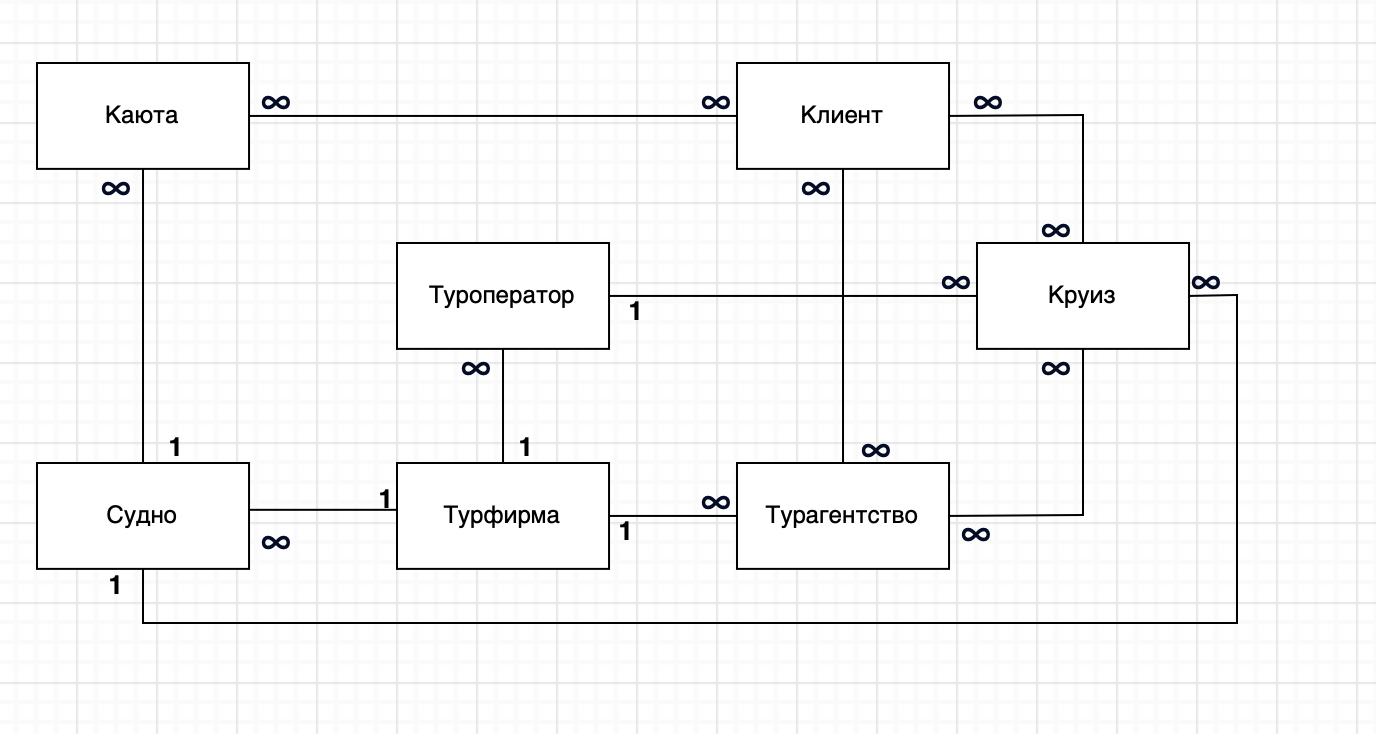
\includegraphics[width=1\textwidth]{5.png}
        \caption{Схема связи сущностей}
        \label{fig:object_relation_schema}
\end{figure}

\newpage
\section{Проектирование}

\subsection{Лингвистическое описание}
\begin{itemize}
\item Круиз(<круиз\_id, INT>, <круиз\_тип\_круиза\_id, INT>, <круиз\_дата, DATE>, <Круиз\_название, VARCHAR(100)>, <круиз\_наполненность, INT>,<туроператор\_id, INT>)
\item Клиент(<клиент\_id, INT>, <клиент\_ФИО, VARCHAR(150)>, <клиент\_история, INT>, <клиент\_личные\_данные, INT>, <клиент\_номер\_каюты, VARCHAR(10)>) 
\item Турфирма(<турфирма\_id, INT>, <турфирма\_название, VARCHAR(100)>, <судно\_id, INT>, <клиент\_id, INT>, <круиз\_id, INT>)
\item Судно(<судно\_id, INT>, <каюта\_id, INT>, <судно\_вместительность, INT>, <судно\_название, VARCHAR(100)>, <судно\_количество\_кают, INT>, <турфирма\_id, INT>, <судно\_тип\_судна\_id, INT>)
\item Каюта(<каюта\_id, INT>, <каюта\_тип\_каюты\_id, INT>, <судно\_id, INT>) 
\item Турагенство(<турагенство\_id, INT>, <турагенство\_название, VARCHAR(100)>, <турфирма\_id, INT>) 
\item Туроператор(<туроператор\_id, INT>, <туроператор\_название, INT>, <туроператор\_название, VARCHAR(100)>) 
\item Круиз клиент каюта(<круиз\_клиент\_каюта\_id, INT>,  <круиз\_id, INT>, <клиент\_id, INT>, <каюта\_id, INT>)
\item Клиент турагенство(<клиент\_турагенство\_id, INT>, <клиент\_id, INT>, <турагенство\_id, INT>) 
\item Круиз турагенство(<круиз\_турагенство\_id, INT>, <круиз\_id, INT>, <турагенство\_id, INT>) 
\item Тип круиза(<тип\_круиза\_id, INT>, <тип\_круиза\_название, VARCHAR(50)>)
\item Тип судно(<тип\_судно\_id, INT>, <тип\_судно\_классификация, VARCHAR(50)>)
\item Тип каюты(<тип\_каюты\_id, INT>, <тип\_каюты\_уровень, VARCHAR(50)>)
\end{itemize}

\newpage
\begin{landscape}
    \ClearShipoutPicture % Очищаем предыдущие элементы
    \AddToShipoutPicture*{%
        \put(\dimexpr 0.5\paperwidth + 9cm, 15cm){ % Ваши точные координаты
            \rotatebox{90}{\thepage} % Повернутый номер
        }%
    }
    \thispagestyle{empty}
\subsection{Таблицы}

\centering

\textbf{Таблица: Круиз (Cruise)}

\begin{longtable}{|p{4cm}|p{3cm}|p{2.6cm}|p{1cm}|p{1cm}|p{5.5cm}|}
\hline
Имя атрибута (рус) & Имя атрибута (англ) & Тип данных & NULL & Ключ & Ссылка \\ \hline
\endhead

круиз\_id & cruise\_id & INT & - & PK & \\ \hline
круиз\_тип\_круиза\_id & cruise\_type\_id & INT & - & FK & CruiseType(cruise\_type\_id) \\ \hline
круиз\_дата & cruise\_date & DATE & - & - & \\ \hline
круиз\_название & cruise\_name & VARCHAR(100) & - & - & \\ \hline
судно\_id & vessel\_id & INT & - & FK & Vessel(vessel\_id) \\ \hline
круиз\_наполненность & cruise\_capacity & INT & NULL & - & \\ \hline
туроператор\_id & tour\_operator\_id & INT & - & FK & TourOperator(tour\_operator\_id) \\ \hline

\caption{Круиз}
\end{longtable}

\textbf{Таблица: Клиент (Client)}

\begin{longtable}{|p{4.3cm}|p{4cm}|p{2.6cm}|p{1cm}|p{1cm}|p{2cm}|}
\hline
Имя атрибута (рус) & Имя атрибута (англ) & Тип данных & NULL & Ключ & Ссылка \\ \hline
\endhead

клиент\_id & client\_id & INT & - & PK & \\ \hline
клиент\_ФИО & client\_full\_name & VARCHAR(150) & - & - & \\ \hline
клиент\_история & client\_history & TEXT & NULL & - & \\ \hline
клиент\_личные\_данные & client\_personal\_data & TEXT & NULL & - & \\ \hline
клиент\_номер\_каюты & client\_cabin\_number & VARCHAR(10) & NULL & - & \\ \hline

\caption{Клиент}
\end{longtable}

\newpage
    \ClearShipoutPicture % Очищаем предыдущие элементы
    \AddToShipoutPicture*{%
        \put(\dimexpr 0.5\paperwidth + 9cm, 15cm){ % Ваши точные координаты
            \rotatebox{90}{\thepage} % Повернутый номер
        }%
    }
    \thispagestyle{empty}
\textbf{Таблица: Турфирма (TravelAgency)}

\begin{longtable}{|p{4cm}|p{3cm}|p{2.6cm}|p{1cm}|p{1cm}|p{3cm}|}
\hline
Имя атрибута (рус) & Имя атрибута (англ) & Тип данных & NULL & Ключ & Ссылка \\ \hline
\endhead

турфирма\_id & agency\_id & INT & - & PK & \\ \hline
турфирма\_название & agency\_name & VARCHAR(100) & - & - & \\ \hline
судно\_id & vessel\_id & INT & NULL & FK & Vessel(vessel\_id) \\ \hline
клиент\_id & client\_id & INT & NULL & FK & Client(client\_id) \\ \hline
круиз\_id & cruise\_id & INT & NULL & FK & Cruise(cruise\_id) \\ \hline

\caption{Турфирма}
\end{longtable}

\textbf{Таблица: Судно (Vessel)}

\begin{longtable}{|p{4.2cm}|p{3.3cm}|p{2.6cm}|p{1cm}|p{1cm}|p{5cm}|}
\hline
Имя атрибута (рус) & Имя атрибута (англ) & Тип данных & NULL & Ключ & Ссылка \\ \hline
\endhead

судно\_id & vessel\_id & INT & - & PK & \\ \hline
каюта\_id & cabin\_id & INT & NULL & FK & Cabin(cabin\_id) \\ \hline
судно\_вместительность & vessel\_capacity & INT & - & - & \\ \hline
судно\_название & vessel\_name & VARCHAR(100) & - & - & \\ \hline
судно\_количество\_кают & vessel\_cabins\_count & INT & - & - & \\ \hline
турфирма\_id & agency\_id & INT & NULL & FK & TravelAgency(agency\_id) \\ \hline
судно\_тип\_судна\_id & vessel\_type\_id & INT & - & FK & VesselType(vessel\_type\_id) \\ \hline

\caption{Судно}
\end{longtable}

\newpage
    \ClearShipoutPicture % Очищаем предыдущие элементы
    \AddToShipoutPicture*{%
        \put(\dimexpr 0.5\paperwidth + 9cm, 15cm){ % Ваши точные координаты
            \rotatebox{90}{\thepage} % Повернутый номер
        }%
    }
    \thispagestyle{empty}
\textbf{Таблица: Каюта (Cabin)}

\begin{longtable}{|p{4cm}|p{3cm}|p{1cm}|p{1cm}|p{1cm}|p{5cm}|}
\hline
Имя атрибута (рус) & Имя атрибута (англ) & Тип данных & NULL & Ключ & Ссылка \\ \hline
\endhead

каюта\_id & cabin\_id & INT & - & PK & \\ \hline
каюта\_тип\_каюты\_id & cabin\_type\_id & INT & - & FK & CabinType(cabin\_type\_id) \\ \hline
судно\_id & vessel\_id & INT & - & FK & Vessel(vessel\_id) \\ \hline

\caption{Каюта}
\end{longtable}

\textbf{Таблица: Турагенство (TourAgency)}

\begin{longtable}{|p{4cm}|p{3.2cm}|p{2.6cm}|p{1cm}|p{1cm}|p{4.3cm}|}
\hline
Имя атрибута (рус) & Имя атрибута (англ) & Тип данных & NULL & Ключ & Ссылка \\ \hline
\endhead

турагенство\_id & tour\_agency\_id & INT & - & PK & \\ \hline
турагенство\_название & tour\_agency\_name & VARCHAR(100) & - & - & \\ \hline
турфирма\_id & agency\_id & INT & NULL & FK & TravelAgency(agency\_id) \\ \hline

\caption{Турагенство}
\end{longtable}

\textbf{Таблица: Туроператор (TourOperator)}

\begin{longtable}{|p{4cm}|p{3.4cm}|p{2.6cm}|p{1cm}|p{1cm}|p{4.2cm}|}
\hline
Имя атрибута (рус) & Имя атрибута (англ) & Тип данных & NULL & Ключ & Ссылка \\ \hline
\endhead

туроператор\_id & tour\_operator\_id & INT & - & PK & \\ \hline
турфирма\_id & agency\_id & INT & NULL & FK & TravelAgency(agency\_id) \\ \hline
туроператор\_название & tour\_operator\_name & VARCHAR(100) & - & - & \\ \hline

\caption{Туроператор}
\end{longtable}

\newpage
    \ClearShipoutPicture % Очищаем предыдущие элементы
    \AddToShipoutPicture*{%
        \put(\dimexpr 0.5\paperwidth + 9cm, 15cm){ % Ваши точные координаты
            \rotatebox{90}{\thepage} % Повернутый номер
        }%
    }
    \thispagestyle{empty}
\textbf{Таблица: Круиз клиент каюта (CruiseClientCabin)}

\begin{longtable}{|p{4.7cm}|p{4cm}|p{1.4cm}|p{1cm}|p{1cm}|p{3.5cm}|}
\hline
Имя атрибута (рус) & Имя атрибута (англ) & Тип данных & NULL & Ключ & Ссылка \\ \hline
\endhead

круиз\_клиент\_каюта\_id & cruise\_client\_cabin\_id & INT & - & PK & \\ \hline
круиз\_id & cruise\_id & INT & - & FK & Cruise(cruise\_id) \\ \hline
клиент\_id & client\_id & INT & - & FK & Client(client\_id) \\ \hline
каюта\_id & cabin\_id & INT & - & FK & Cabin(cabin\_id) \\ \hline

\caption{Круиз клиент каюта}
\end{longtable}

\textbf{Таблица: Клиент турагенство (ClientTourAgency)}

\begin{longtable}{|p{4.2cm}|p{4cm}|p{1.4cm}|p{1cm}|p{1cm}|p{5.2cm}|}
\hline
Имя атрибута (рус) & Имя атрибута (англ) & Тип данных & NULL & Ключ & Ссылка \\ \hline
\endhead

клиент\_турагенство\_id & client\_tour\_agency\_id & INT & - & PK & \\ \hline
клиент\_id & client\_id & INT & - & FK & Client(client\_id) \\ \hline
турагенство\_id & tour\_agency\_id & INT & - & FK & TourAgency(tour\_agency\_id) \\ \hline

\caption{Клиент турагенство}
\end{longtable}


\textbf{Таблица: Круиз турагенство (CruiseTourAgency)}

\begin{longtable}{|p{4cm}|p{4cm}|p{1.4cm}|p{1cm}|p{1cm}|p{5.5cm}|}
\hline
Имя атрибута (рус) & Имя атрибута (англ) & Тип данных & NULL & Ключ & Ссылка \\ \hline
\endhead

круиз\_турагенство\_id & cruise\_tour\_agency\_id & INT & - & PK & \\ \hline
круиз\_id & cruise\_id & INT & - & FK & Cruise(cruise\_id) \\ \hline
турагенство\_id & tour\_agency\_id & INT & - & FK & TourAgency(tour\_agency\_id) \\ \hline

\caption{Круиз турагенство}
\end{longtable}
\end{landscape}

\newpage
\textbf{Таблица: Тип куриза (CruiseType)}

\begin{longtable}{|p{3.8cm}|p{3cm}|p{2.6cm}|p{1cm}|p{1cm}|p{2cm}|}
\hline
Имя атрибута (рус) & Имя атрибута (англ) & Тип данных & NULL & Ключ & Ссылка \\ \hline
\endhead

тип\_куриза\_id & cruise\_type\_id & INT & - & PK & \\ \hline
тип\_куриза\_название & cruise\_type\_name & VARCHAR(100) & - & - & \\ \hline

\caption{Тип куриза}
\end{longtable}

\textbf{Таблица: Тип судна (VesselType)}

\begin{longtable}{|p{4.7cm}|p{3cm}|p{2.6cm}|p{1cm}|p{1cm}|p{2cm}|}
\hline
Имя атрибута (рус) & Имя атрибута (англ) & Тип данных & NULL & Ключ & Ссылка \\ \hline
\endhead

тип\_судна\_id & vessel\_type\_id & INT & - & PK & \\ \hline
тип\_судна\_классификация & vessel\_type\_class & VARCHAR(50) & - & - & \\ \hline

\caption{Тип судна}
\end{longtable}

\textbf{Таблица: Тип каюты (CabinType)}

\begin{longtable}{|p{4cm}|p{3cm}|p{2.6cm}|p{1cm}|p{1cm}|p{2cm}|}
\hline
Имя атрибута (рус) & Имя атрибута (англ) & Тип данных & NULL & Ключ & Ссылка \\ \hline
\endhead

тип\_каюты\_id & cabin\_type\_id & INT & - & PK & \\ \hline
тип\_каюты\_уровень & cabin\_type\_level & VARCHAR(50) & - & - & \\ \hline

\caption{Тип каюты}
\end{longtable}

\vspace{60pt}{
Персональные ключи имеют тип INT, чтобы с добавлением записи в базу
данных идентификаторы автоматически увеличивались. Фамилия, имя и
отчество хранятся в строке длины до 150 символов, чего должно хватить для двойных имен и фамилий. Все названия хранятся в строке длины до 100 символов, так как все названия должны хорошо запоминаться и не должны состоять из множества слов. Для перечня заранее известных слов выделена строка из 50 символов, таких как классификация и уровень каюты. Они известны заванее и использоваться может строка из 15 символов, однако учитывается случай добавления новых компонент. Все таблицы перечисленны выше.}

\newpage
\subsection{Схемы баз данных}
Отчет содержит две схемы баз данных: русскоязычную (Рис. 4) и англоязычную версию (Рис. 5). Наличие русскоязычного варианта облегчает восприятие структуры для тех, кто работает с предметной областью на русском языке, а англоязычная схема соответствует международным стандартам именования в IT-проектах. Обе диаграммы отражают идентичную логическую структуру базы данных, спроектированную для системы бронирования круизов.

Также реализована схема заполнения базы данных (см. Рис.~\ref{fig:por_soz}).
\\
\begin{figure}[h]
     	\centering
     	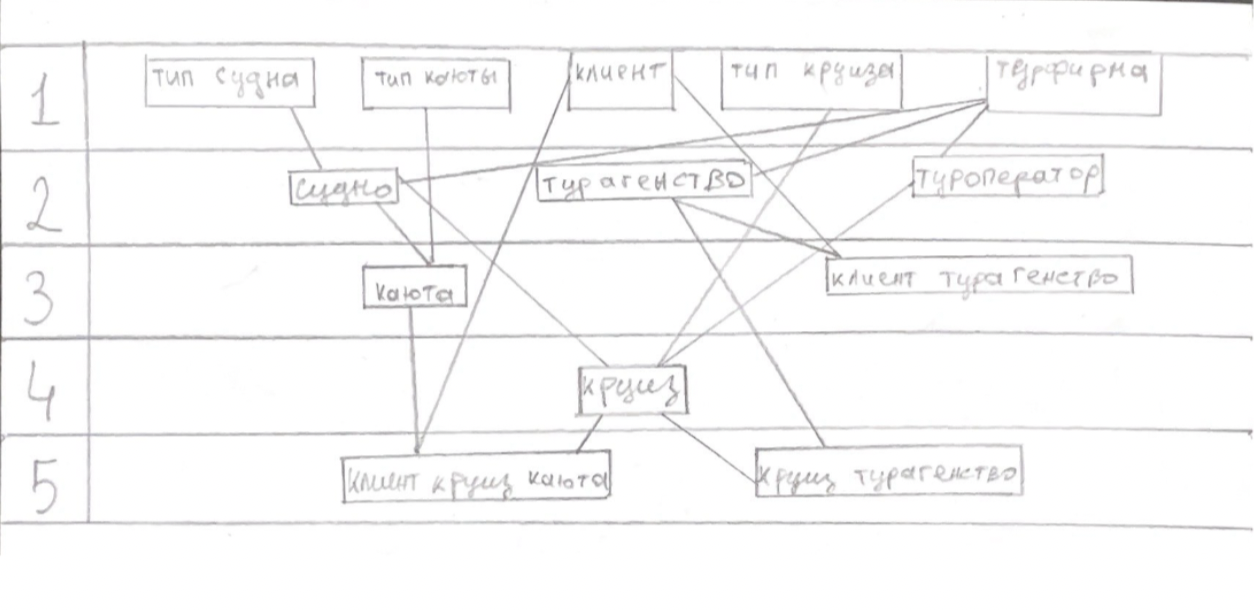
\includegraphics[width=1\textwidth]{39.png}
        \caption{Порядок создания таблиц}
        \label{fig:por_soz}
\end{figure}

\newpage
\includepdf[
    pages=-,
    landscape,
    fitpaper=true,
    offset=0 0,
    scale=1,
    pagecommand={
        \thispagestyle{empty} % Полностью отключаем номер страницы
        \begin{tikzpicture}[remember picture, overlay]
            % Только подпись "Рис.3" внизу по центру
            \node[anchor=south, rotate=90, xshift=0cm, yshift=2.5cm] at (current page.east) {
                \large\textbf{Рис. 4. Схема базы данных на русском языке}
            };
            \node[anchor=south, rotate=90, xshift=0cm, yshift=1.5cm] at (current page.east) { % Пробуем якорь .east
                \thepage
            };
        \end{tikzpicture}
    }
]{3.pdf}

\addtocounter{figure}{1}
\addtocounter{figure}{1}

\newpage
\includepdf[
    pages=-,
    landscape,
    fitpaper=true,
    offset=0 0,
    scale=1,
    pagecommand={
        \thispagestyle{empty} % Полностью отключаем номер страницы
        \begin{tikzpicture}[remember picture, overlay]
            % Только подпись "Рис.3" внизу по центру
            \node[anchor=south, rotate=90, xshift=0cm, yshift=2.5cm] at (current page.east) {
                \large\textbf{Рис. 5. Схема базы данных на английском языке}
            };
            \node[anchor=south, rotate=90, xshift=0cm, yshift=1.5cm] at (current page.east) { % Пробуем якорь .east
                \thepage
            };
        \end{tikzpicture}
    }
]{9.pdf}

\newpage
\section{Программирование}
\begin{figure}[h!]
    \centering
    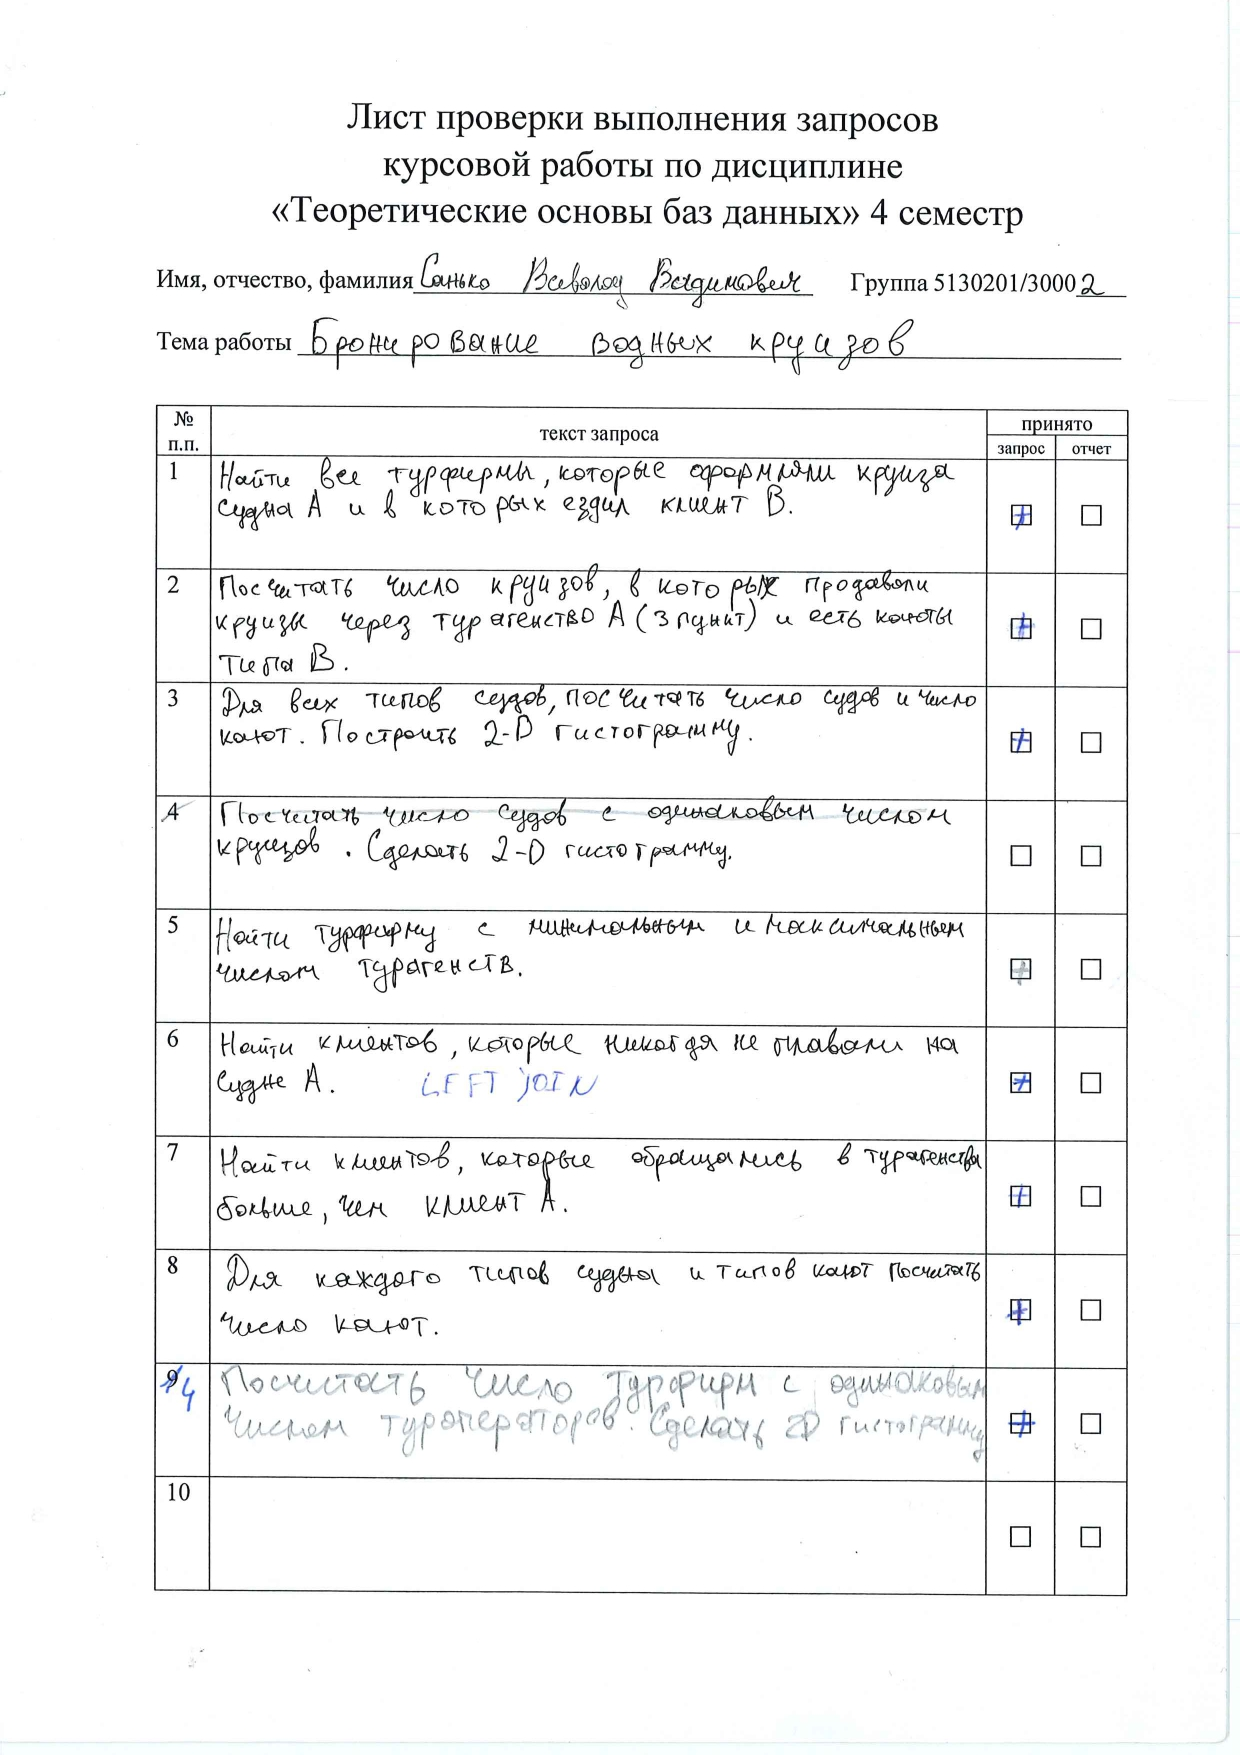
\includegraphics[width=0.95\textwidth]{42.jpg} 
\end{figure}


\newpage
\Large\textbf{{Выполнение запросов}}
\subsection{Запрос 1}
{
Найти все турфирмы, которые оформляли круизы судна А и в котором ездил клиент Б.
}
\begin{lstlisting}[style=sqlstyle, label=sql:query1]
SELECT DISTINCT ta.agency_name AS "Название агентства"
FROM TravelAgency ta
JOIN TourAgency tour_ag ON ta.agency_id = tour_ag.agency_id
JOIN CruiseTourAgency cta ON tour_ag.tour_agency_id = cta.tour_agency_id
JOIN Cruise c ON cta.cruise_id = c.cruise_id
JOIN Vessel v ON c.vessel_id = v.vessel_id
JOIN ClientCruiseCabin b ON c.cruise_id = b.cruise_id
JOIN Client cl ON b.client_id = cl.client_id
WHERE v.vessel_name = 'Ветер'
  AND cl.client_full_name = 'Попова Полина Павеловна';
\end{lstlisting}
\begin{figure}[h!]
    \centering
    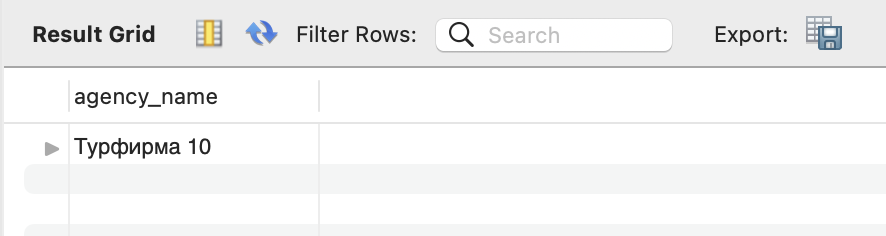
\includegraphics[width=0.7\textwidth]{10.png} 
    \caption{Результаты запроса 1}
\end{figure}
{\centeringВремя выполнения запроса: 0:00:0.010.\par}
\begin{figure}[H]
    \centering
    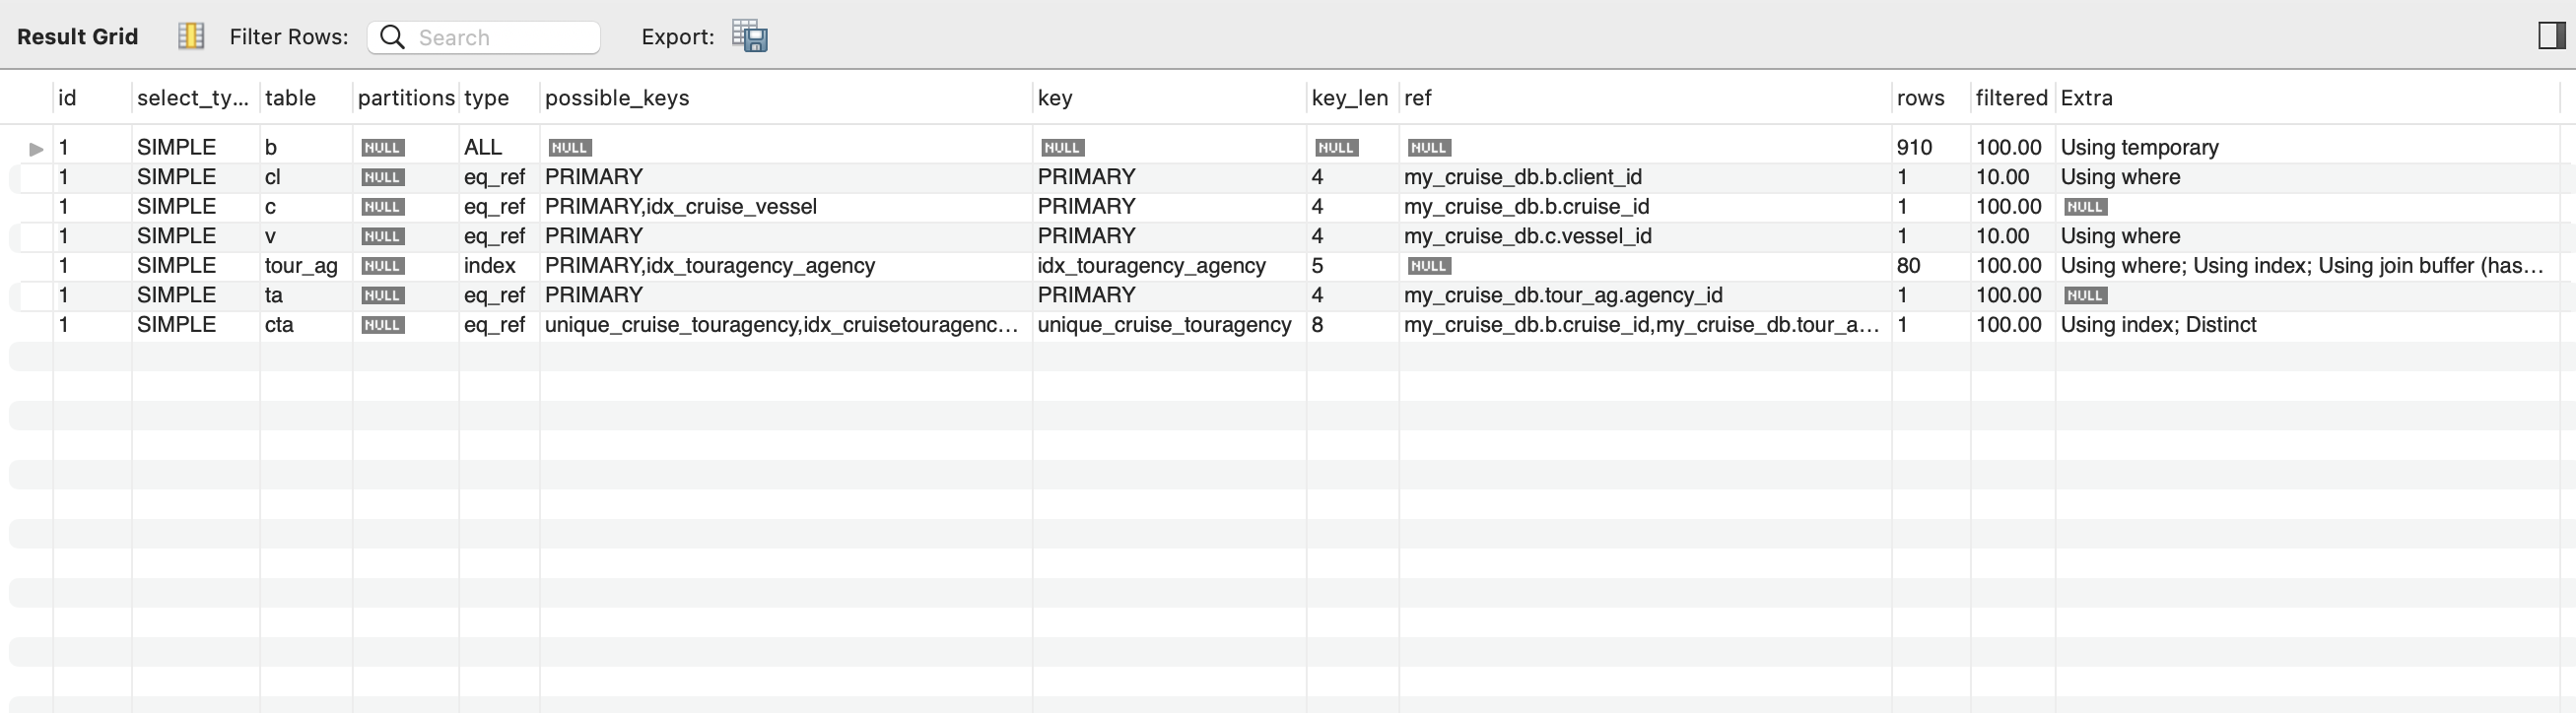
\includegraphics[width=0.7\textwidth]{11.png} 
    \caption{Explain запроса 1}
\end{figure}

Запрос находит все турагентства, которые организовывали круизы на судне "Ветер" для клиента Попова П.П. Соединяет 7 таблиц (от клиентов до судов) через INNER JOIN, что гарантирует точное соответствие условиям поиска.
\\
\\
\\
$$
\pi_{\text{ta.agency\_name}} \Bigg(
  \sigma_{\begin{subarray}{l}
    \text{v.vessel\_name} = \text{'Ветер'} \\ 
    \wedge\ \text{cl.client\_full\_name} = \text{'Попова Полина Павеловна'}
  \end{subarray}} \Bigg(
$$

$$
  \begin{aligned}
    &\beta_{\text{ta}}(\text{TravelAgency}) \\
    &\bowtie_{\text{ta.agency\_id} = \text{tour\_ag.agency\_id}} \beta_{\text{tour\_ag}}(\text{TourAgency}) \\
    &\bowtie_{\text{tour\_ag.tour\_agency\_id} = \text{cta.tour\_agency\_id}} \beta_{\text{cta}}(\text{CruiseTourAgency}) \\
    &\bowtie_{\text{cta.cruise\_id} = \text{c.cruise\_id}} \beta_{\text{c}}(\text{Cruise}) \\
    &\bowtie_{\text{c.vessel\_id} = \text{v.vessel\_id}} \beta_{\text{v}}(\text{Vessel}) \\
    &\bowtie_{\text{c.cruise\_id} = \text{b.cruise\_id}} \beta_{\text{b}}(\text{ClientCruiseCabin}) \\
    &\bowtie_{\text{b.client\_id} = \text{cl.client\_id}} \beta_{\text{cl}}(\text{Client})
  \end{aligned} \Bigg) \Bigg)
$$

\subsection{Запрос 2}
Посчитать число круизов в которых продавали круизы через турагенство А(использовать поле турагенство\_название) и есть каюты типа Б.
\begin{lstlisting}[style=sqlstyle, label=sql:query1]
SELECT COUNT(DISTINCT c.cruise_id) AS total_cruises
FROM Cruise c
JOIN CruiseTourAgency cta ON c.cruise_id = cta.cruise_id
JOIN TourAgency ta ON cta.tour_agency_id = ta.tour_agency_id
JOIN Cabin cab ON c.vessel_id = cab.vessel_id
JOIN CabinType ct ON cab.cabin_type_id = ct.cabin_type_id
WHERE ta.tour_agency_name = 'Турагентство 72' 
  AND ct.cabin_type_level = 'Люкс'; 
\end{lstlisting}
\begin{figure}[h!]
    \centering
    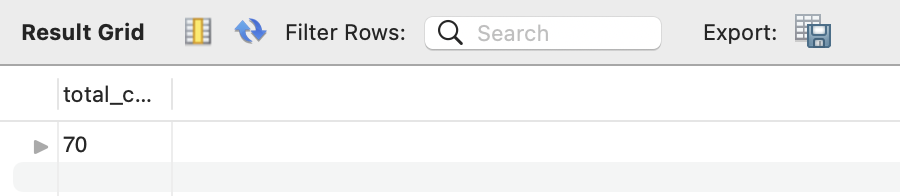
\includegraphics[width=0.6\textwidth]{12.png} 
    \caption{Результаты запроса 2}
\end{figure}
{\centering
Время выполнения запроса: 0:00:0.0052.\par}
\begin{figure}[H]
    \centering
    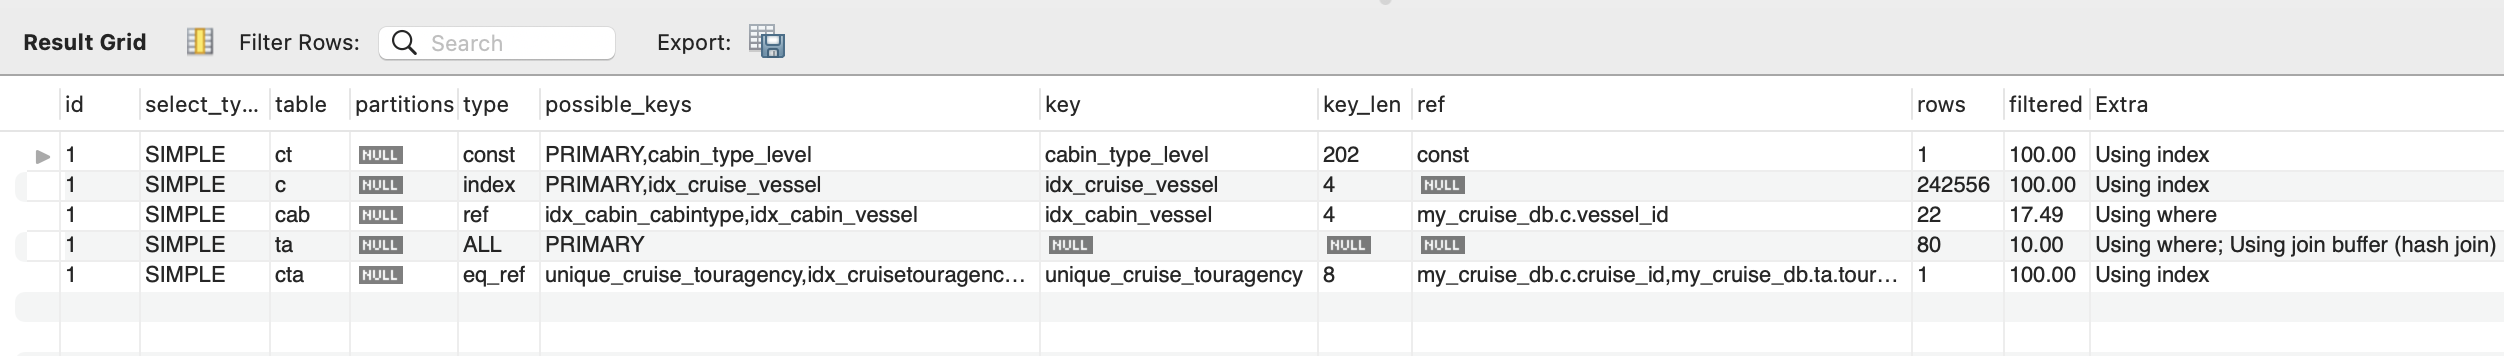
\includegraphics[width=\textwidth]{13.png} 
    \caption{Explain запроса 2}
\end{figure}

Вычисляет количество уникальных круизов, продававшихся через "Турагентство 72", где были доступны каюты класса "Люкс". Использует \newline 
COUNT(DISTINCT) для исключения дублирования круизов в статистике.

$$
\gamma(\text{COUNT(DISTINCT c.cruise\_id)})(\delta(
$$
$$
\text{Cruise c} \bowtie \text{CruiseTourAgency cta} \bowtie
$$
$$
\text{TourAgency ta} \bowtie \text{Cabin cab} \bowtie \text{CabinType ct}
$$
$$
\triangle \sigma\begin{pmatrix}
\text{ta.tour\_agency\_name} = \text{'Турагентство 77'} \\
\wedge \text{ct.cabin\_type\_level} = \text{'Люкс'}
\end{pmatrix}
$$
$$))$$

\subsection{Запрос 3}
Для всех типов судов посчитать число судов и число кают. Построить гистограмму.

\begin{lstlisting}[style=sqlstyle, label=sql:query1]
SELECT
    vt.vessel_type_class AS тип_судна,
    COUNT(DISTINCT v.vessel_id) AS количество_судов,
    SUM(v.vessel_cabins_count) AS общее_количество_кают
FROM
    VesselType vt
LEFT JOIN
    Vessel v ON vt.vessel_type_id = v.vessel_type_id
GROUP BY
    vt.vessel_type_class
ORDER BY
    количество_судов DESC;
\end{lstlisting}
\begin{figure}[h!]
    \centering
    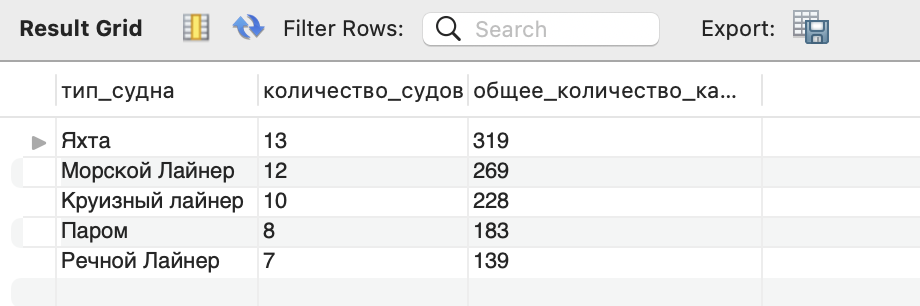
\includegraphics[width=0.7\textwidth]{14.png} 
    \caption{Результаты запроса 3}
\end{figure}
{\centering
Время выполнения запроса: 0:00:1.609.\par}
\begin{figure}[H]
    \centering
    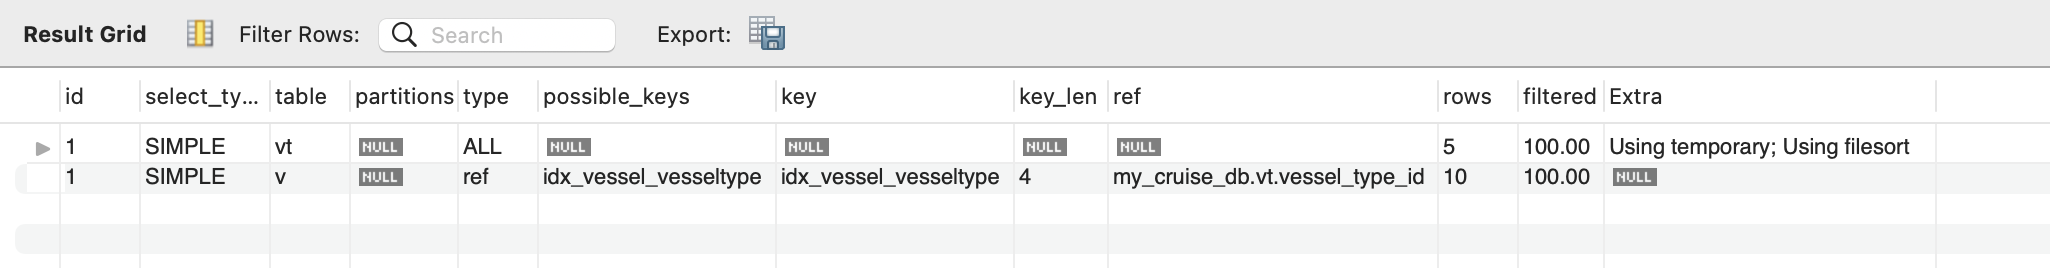
\includegraphics[width=\textwidth]{15.png} 
    \caption{Explain запроса 3}
\end{figure}

Формирует сводную таблицу с количеством судов и общим числом кают для каждого класса судов. LEFT JOIN обеспечивает включение всех типов судов, даже без фактических экземпляров. Результаты сортируются по убыванию количества судов. Ниже представлены визуализация плана выполнения запроса (Рис.\ref{fig:expl3}) и гистограмма (Рис.\ref{fig:hist3}).

$$
\gamma\begin{pmatrix}
\text{vt.vessel\_type\_class}, \\
\text{COUNT(DISTINCT v.vessel\_id)}, \\
\text{SUM(v.vessel\_cabins\_count)}
\end{pmatrix}
$$
$$
\beta_{\text{tv}}(\text{VesselType}) \leftouterjoin \beta_{\text{v}}(\text{Vessel})
$$

\begin{figure}[H]
    \centering
    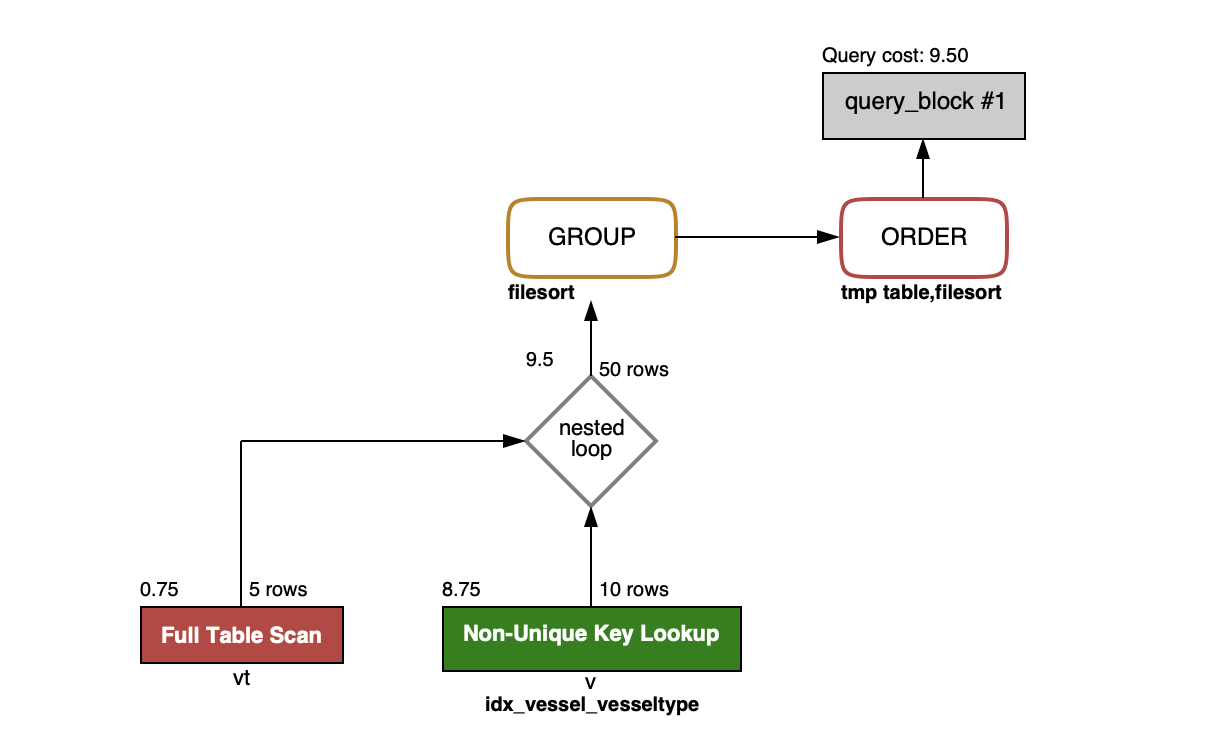
\includegraphics[width=\textwidth]{33.png} 
    \caption{Visual explain запроса 3}
    \label{fig:expl3}
\end{figure}

\newpage
\begin{figure}[h!]
    \centering
    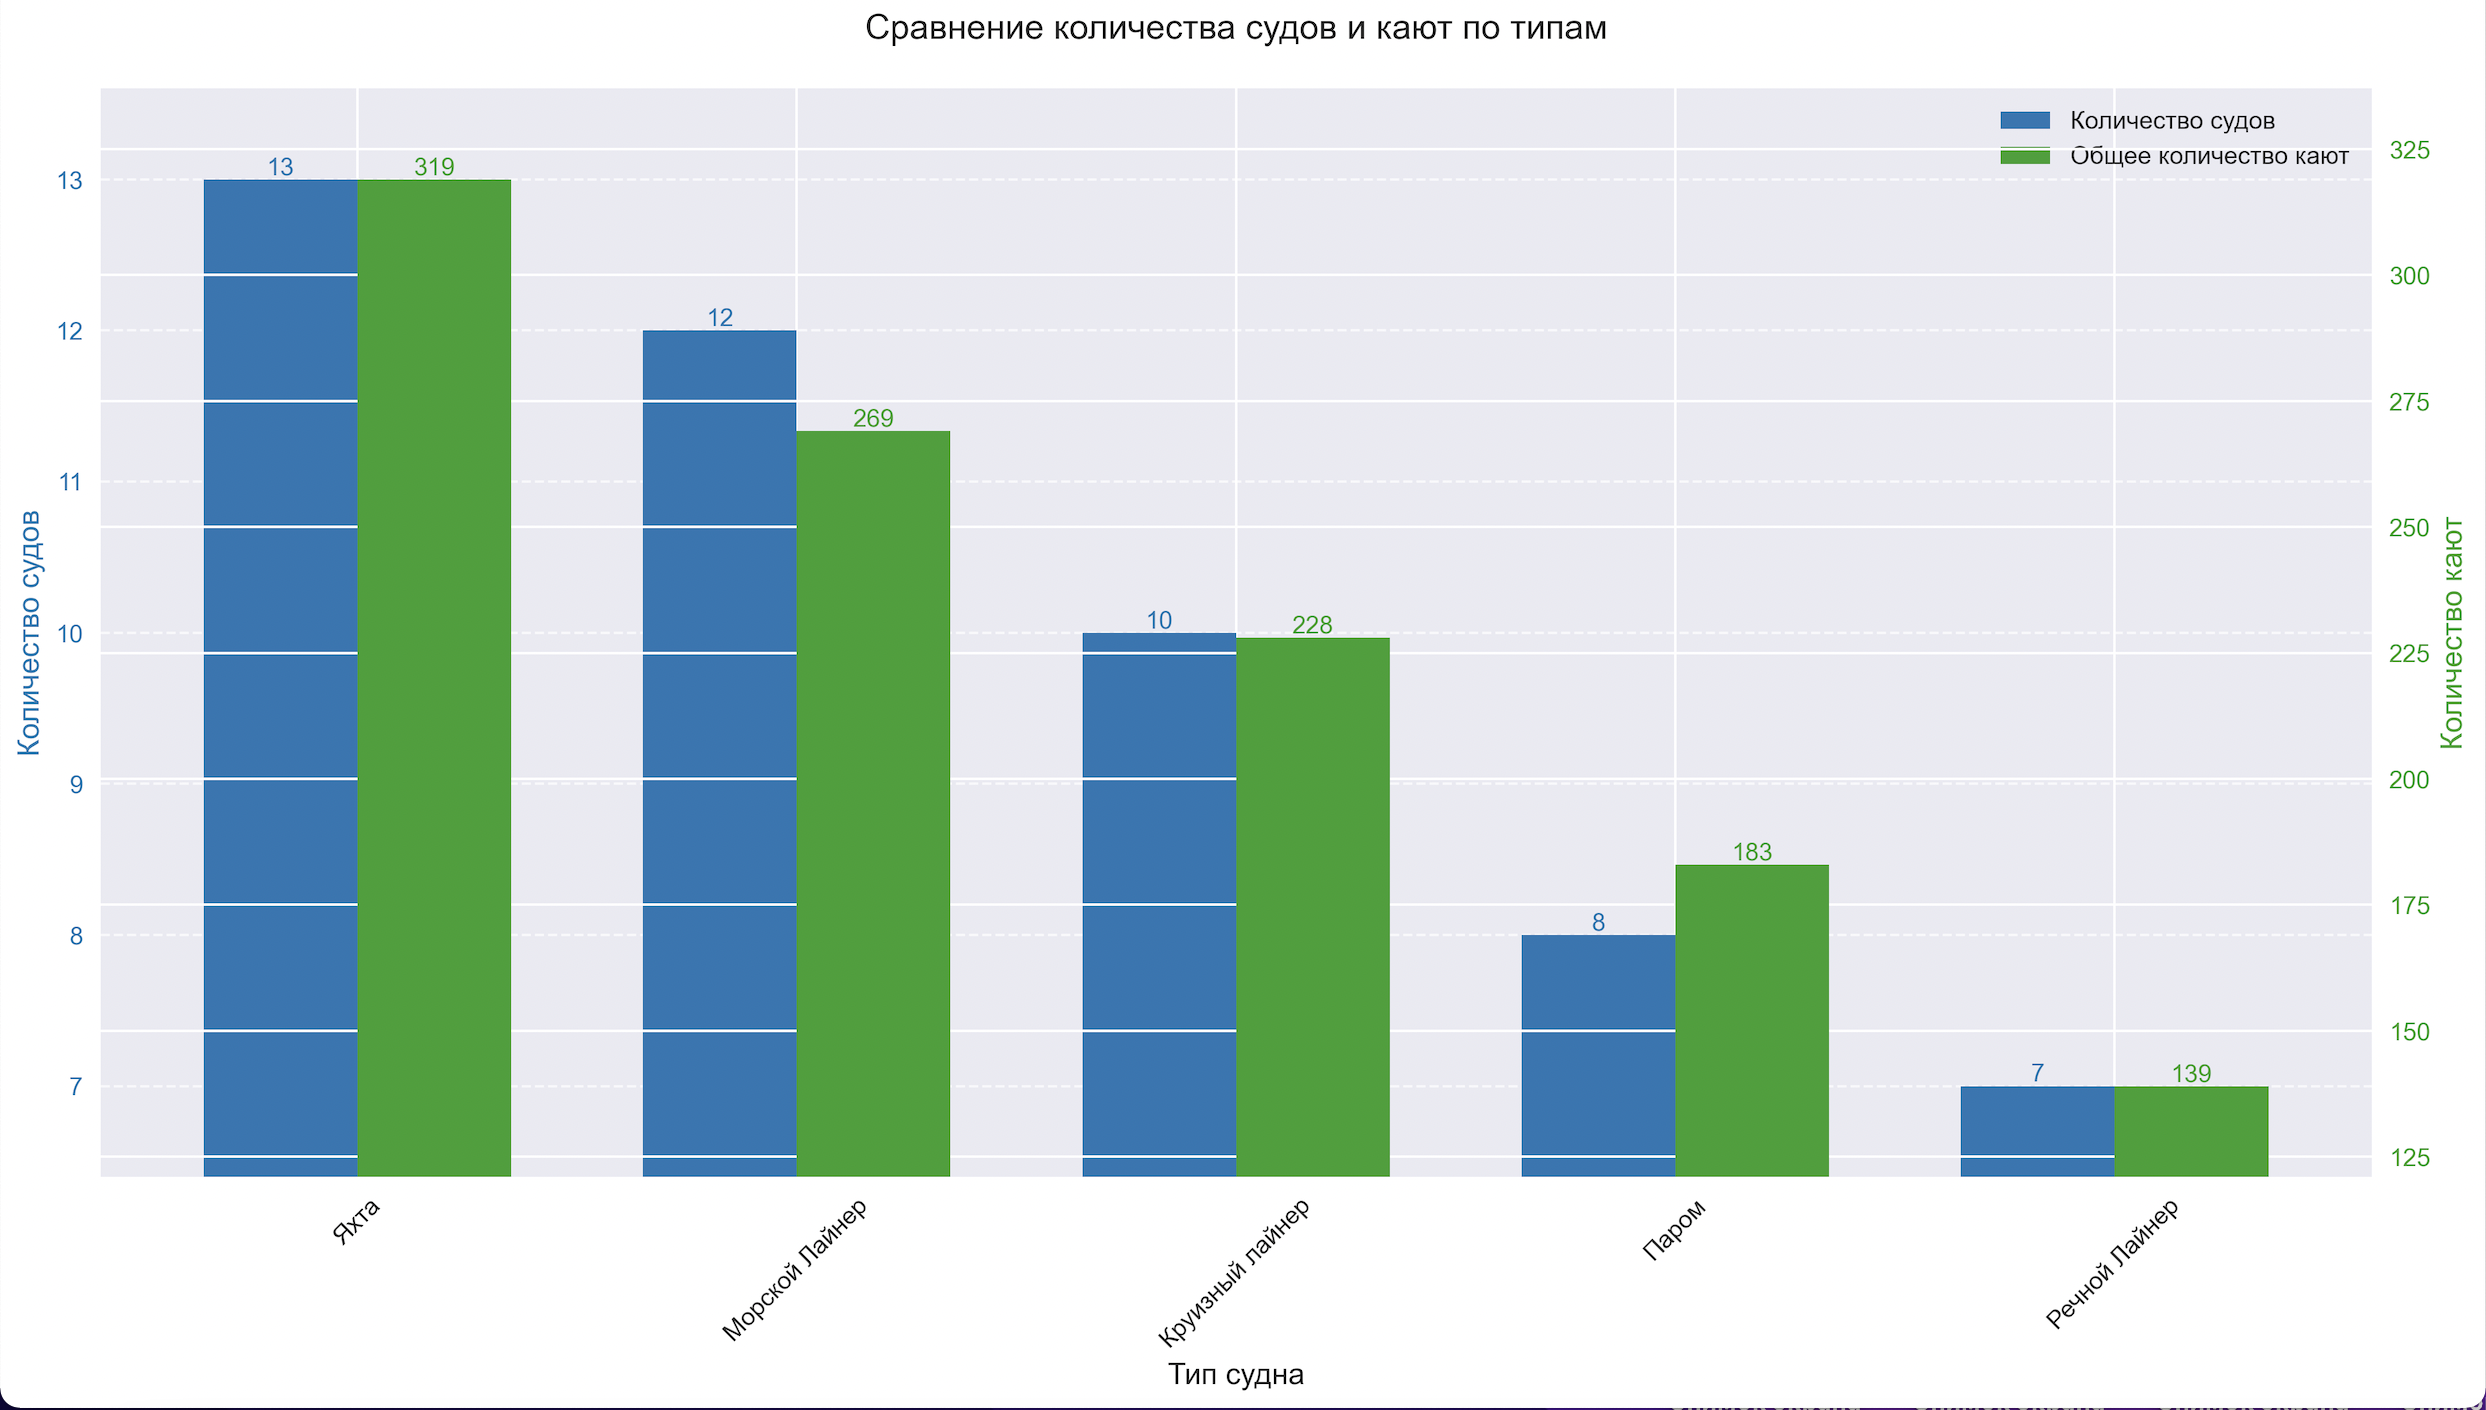
\includegraphics[width=1.05\textwidth]{52.png} 
    \caption{2D гистограмма  запроса 3}
    \label{fig:hist3}
\end{figure}

\subsection{Запрос 4}
Посчитать число турфирм с одинаковым числом туроператоров.
\begin{lstlisting}[style=sqlstyle, label=sql:query1]
SELECT
    operator_count AS количество_туроператоров_в_турфирме,
    COUNT(agency_id) AS количество_таких_турфирм
FROM (
    SELECT
        ta.agency_id,
        COUNT(DISTINCT t_op.tour_operator_id) AS operator_count
    FROM
        TravelAgency ta
    LEFT JOIN
        TourOperator t_op ON ta.agency_id = t_op.agency_id
    GROUP BY
        ta.agency_id
) AS AgencyOperatorCounts
GROUP BY
    operator_count
ORDER BY
    количество_таких_турфирм DESC, количество_туроператоров_в_турфирме DESC;
\end{lstlisting}
\begin{figure}[h!]
    \centering
    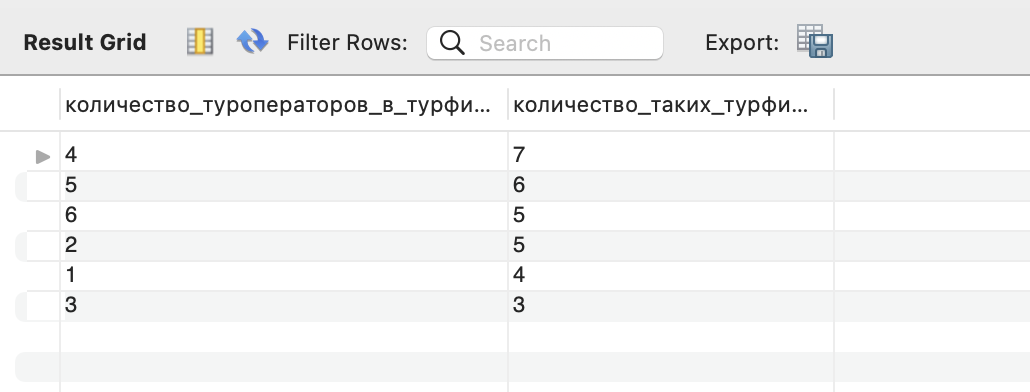
\includegraphics[width=0.55\textwidth]{16.png} 
    \caption{Результаты запроса 4}
\end{figure}
{\centering
Время выполнения запроса: 0:00:0.0026.\par}
\begin{figure}[H]
    \centering
    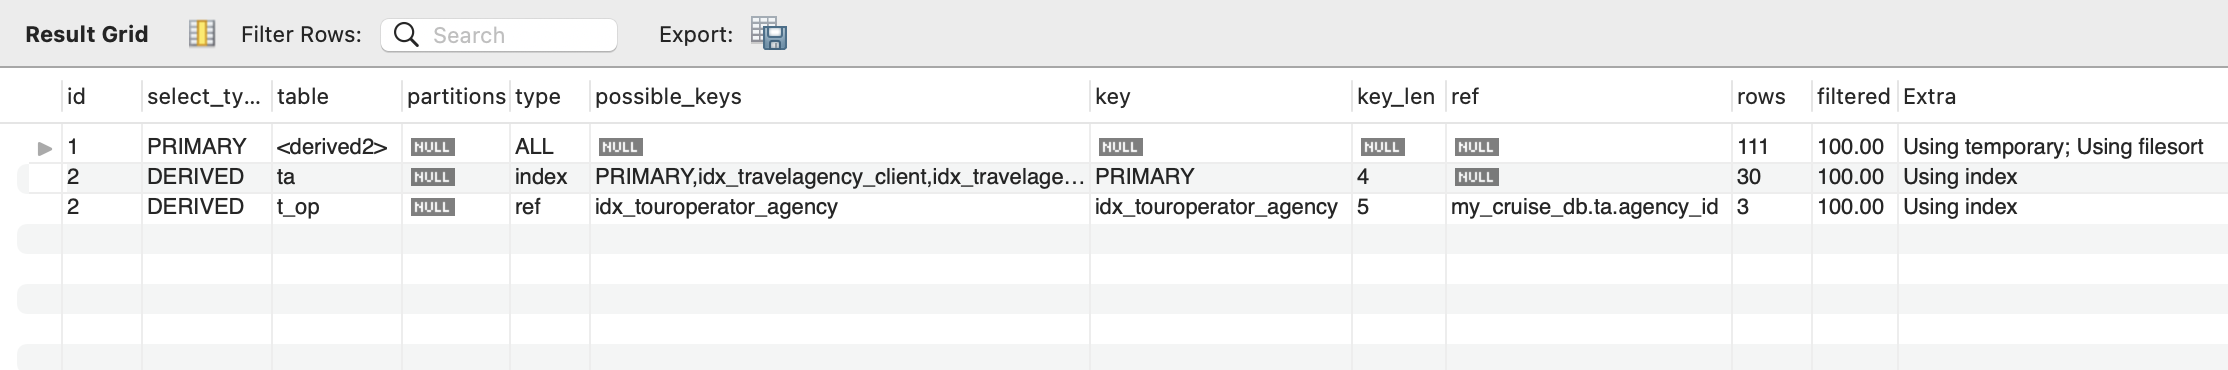
\includegraphics[width=\textwidth]{17.png} 
    \caption{Explain запроса 4}
\end{figure}

Анализирует, сколько турфирм имеет одинаковое количество туроператоров. Вложенный запрос сначала считает туроператоров для каждой турфирмы, затем группирует по этому показателю. Результаты представлены в виде гистограммы на Рис.~\ref{fig:hist4}.

$$
\gamma(\text{cruise\_count}, \text{COUNT(vessel\_id)})(
$$
$$
\gamma(\text{v.vessel\_id}, \text{COUNT(c.cruise\_id) AS cruise\_count})
$$
$$
\beta_{\text{c}}(\text{Cruise}) \leftouterjoin \beta_{\text{v}}(\text{Vessel})
$$

\begin{figure}[H]
    \centering
    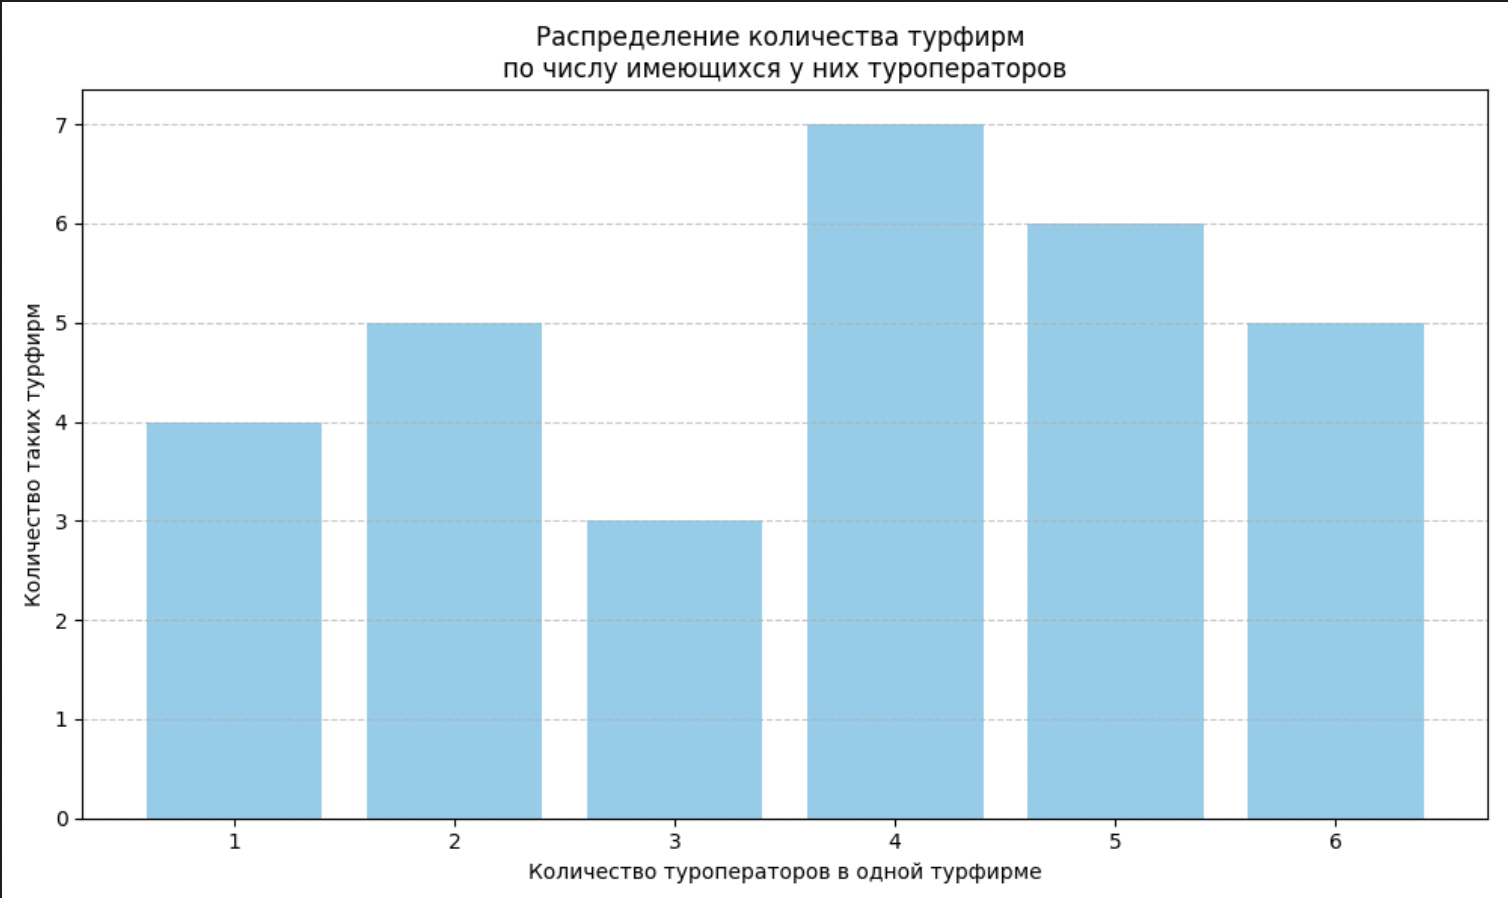
\includegraphics[width=0.7\textwidth]{53.png} 
    \caption{2D гистограмма  запроса 4}
    \label{fig:hist4}
\end{figure}

%\newpage
\subsection{Запрос 5.1}
Найти турфирму с минимальным числом турагенств.
\begin{lstlisting}[style=sqlstyle, label=sql:query1]
SELECT 
    ta.agency_name, 
    COUNT(toura.tour_agency_id) AS number_of_tour_agencies
FROM 
    TravelAgency ta
LEFT JOIN 
    TourAgency toura ON ta.agency_id = toura.agency_id
GROUP BY 
    ta.agency_id, ta.agency_name
HAVING 
    COUNT(toura.tour_agency_id) = (
        SELECT COUNT(toura2.tour_agency_id) AS cnt
        FROM TravelAgency ta2
        LEFT JOIN TourAgency toura2 ON ta2.agency_id = toura2.agency_id
        GROUP BY ta2.agency_id
        ORDER BY cnt ASC
        LIMIT 1
    )
\end{lstlisting}
\begin{figure}[h!]
    \centering
    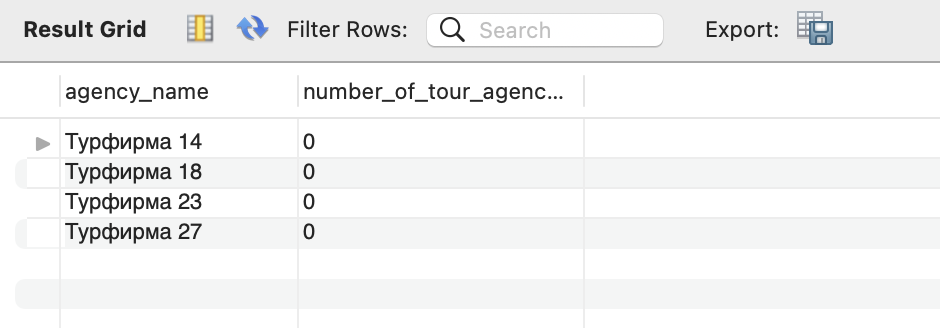
\includegraphics[width=0.6\textwidth]{18.png} 
    \caption{Результаты запроса 5}
\end{figure}
{\centering
Время выполнения запроса: 0:00:0.0064.\par}
\begin{figure}[H]
    \centering
    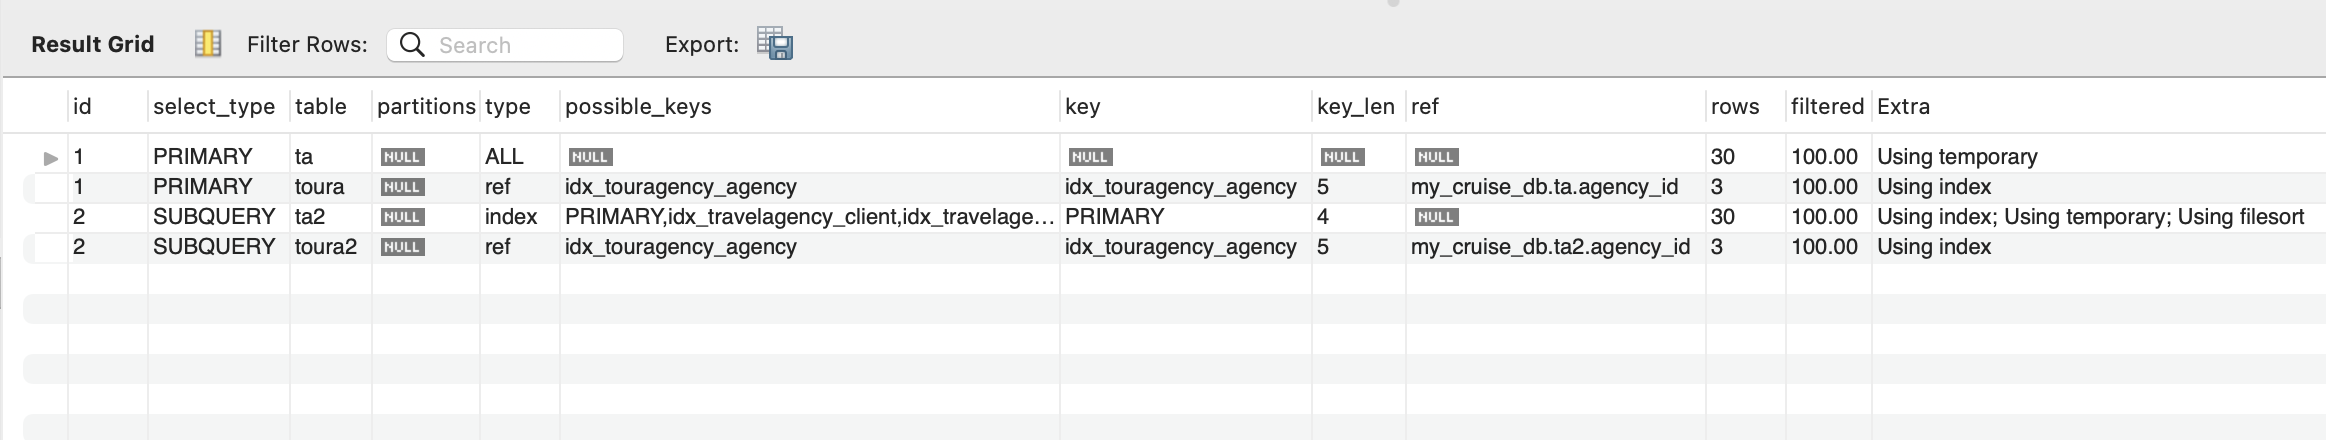
\includegraphics[width=0.9\textwidth]{19.png} 
    \caption{Explain запроса 5}
\end{figure}
\\
$$
\tau_{\text{number\_of\_tour\_agencies ASC}}(
$$
$$
\gamma(\text{ta.agency\_name}, \text{COUNT(toura.tour\_agency\_id) AS number\_of\_tour\_agencies})
$$
$$
\beta_{\text{ta}}(\text{TravelAgency}) \leftouterjoin \beta_{\text{toura}}(\text{TourAgency})
$$


\subsection{Запрос 5.2}
Найти турфирму с максимальным числом турагенств.
\begin{lstlisting}[style=sqlstyle, label=sql:query1]
SELECT 
    ta.agency_name, 
    COUNT(toura.tour_agency_id) AS number_of_tour_agencies
FROM 
    TravelAgency ta
LEFT JOIN 
    TourAgency toura ON ta.agency_id = toura.agency_id
GROUP BY 
    ta.agency_id, ta.agency_name
HAVING 
    COUNT(toura.tour_agency_id) = (
        SELECT COUNT(toura2.tour_agency_id) AS cnt
        FROM TravelAgency ta2
        LEFT JOIN TourAgency toura2 ON ta2.agency_id = toura2.agency_id
        GROUP BY ta2.agency_id
        ORDER BY cnt DESC
        LIMIT 1
    )
\end{lstlisting}
\begin{figure}[h!]
    \centering
    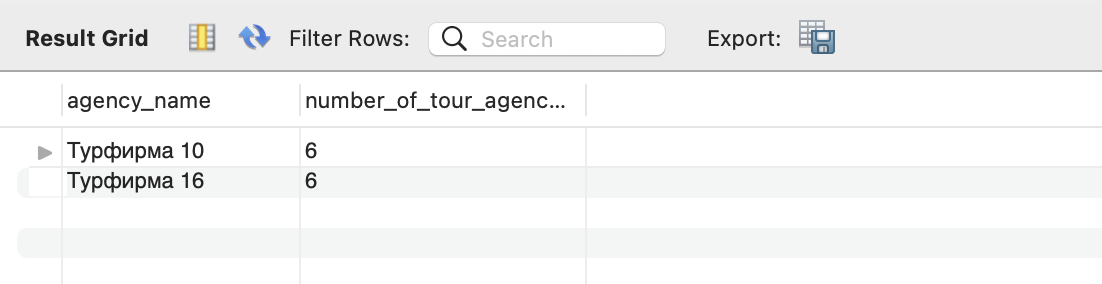
\includegraphics[width=0.7\textwidth]{20.png} 
    \caption{Результаты запроса 5}
\end{figure}
{\centering
Время выполнения запроса: 0:00:0.00091.\par}
\begin{figure}[H]
    \centering
    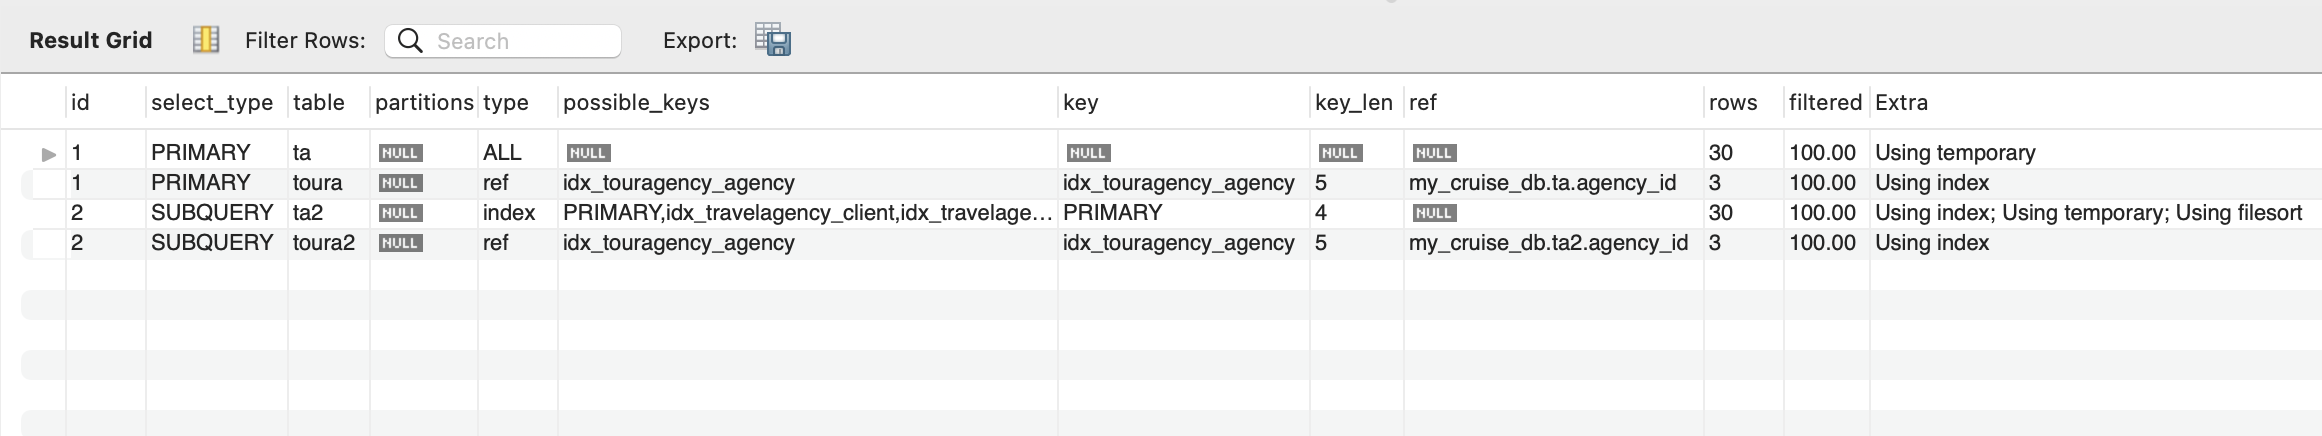
\includegraphics[width=\textwidth]{21.png} 
    \caption{Explain запроса 5}
\end{figure}
\\
$$
\tau_{\text{number\_of\_tour\_agencies DESC}}(
$$
$$
\gamma(\text{ta.agency\_name}, \text{COUNT(toura.tour\_agency\_id) AS number\_of\_tour\_agencies})(
$$
$$
\beta_{\text{ta}}(\text{TravelAgency}) \leftouterjoin \beta_{\text{toura}}(\text{TourAgency})
$$


Два симметричных запроса находят турфирмы с минимальным и максимальным количеством дочерних турагентств. Используют LEFT JOIN для учёта фирм без агентств и LIMIT для вывода одного результата. Запрос был проанализирован с помощью функции VISUAL EXPLAIN (см. Рис.~\ref{fig:expl5}).
\begin{figure}[H]
    \centering
    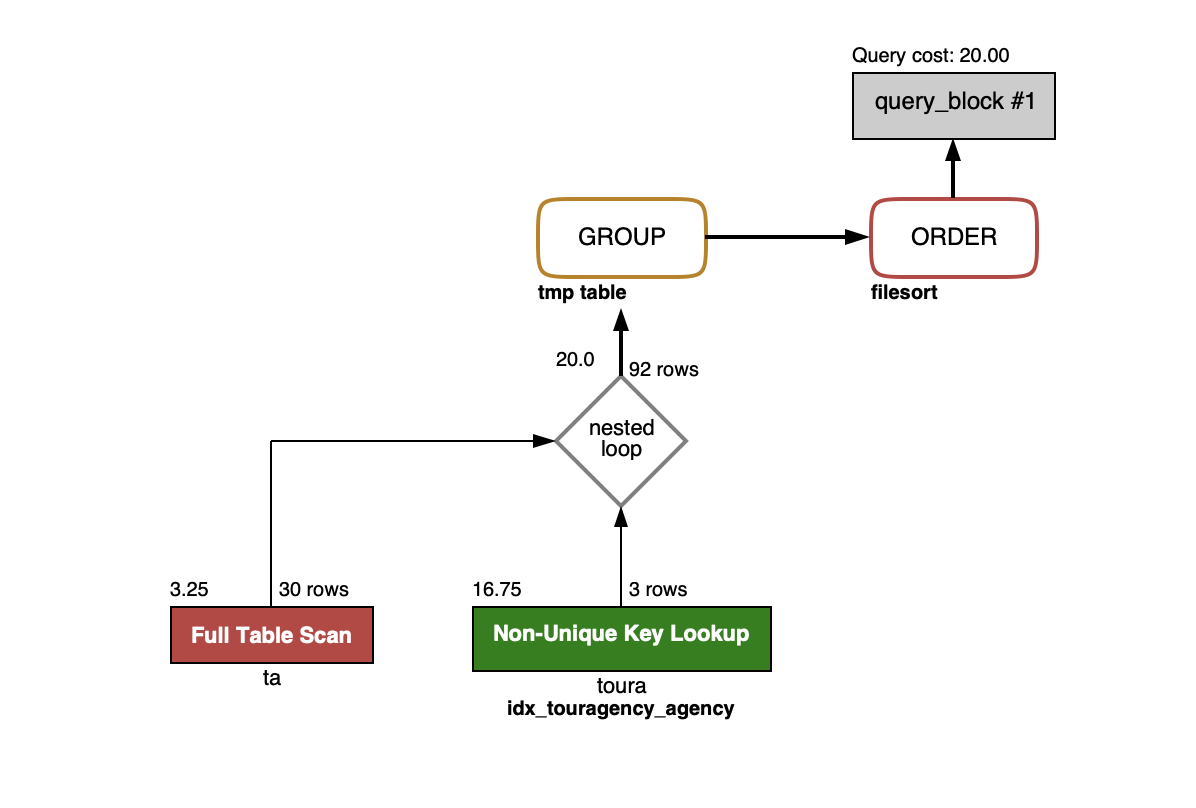
\includegraphics[width=0.9\textwidth]{352.png} 
    \caption{Visual explain запроса 5}
    \label{fig:expl5}
\end{figure}

\subsection{Запрос 6}
Найти клиентов которые никогда не плавали на судне А.
\begin{lstlisting}[style=sqlstyle, label=sql:query1]
SELECT
    c.client_id,
    c.client_full_name
FROM
    Client c
WHERE
    NOT EXISTS (
        SELECT 1
        FROM ClientCruiseCabin b
        JOIN Cruise cr ON b.cruise_id = cr.cruise_id
        JOIN Vessel v ON cr.vessel_id = v.vessel_id
        WHERE v.vessel_name = '"Дух"'
          AND b.client_id = c.client_id 
    );
\end{lstlisting}
\begin{figure}[h!]
    \centering
    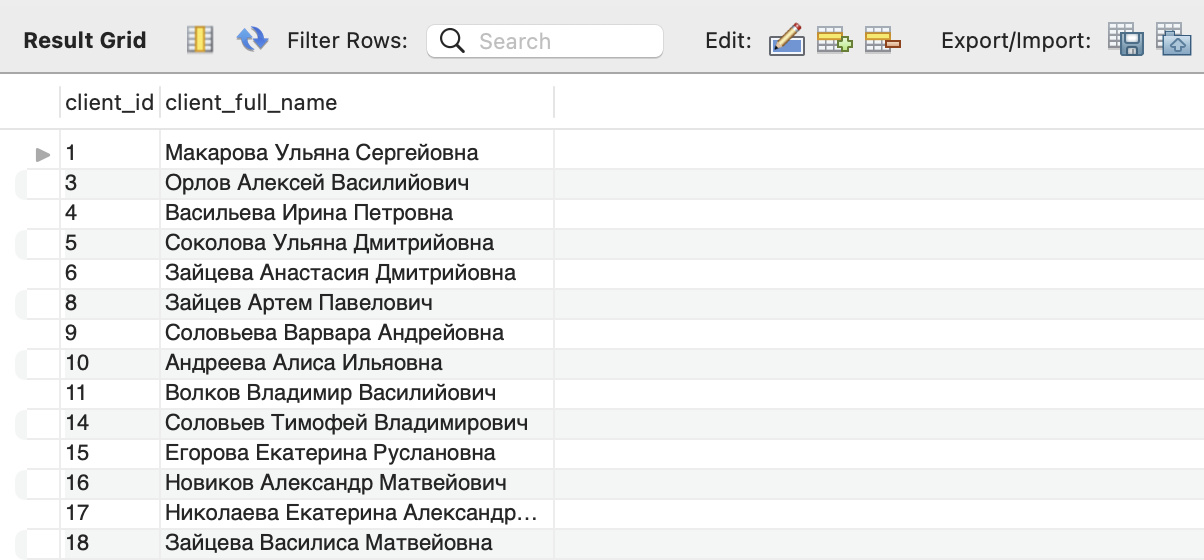
\includegraphics[width=0.9\textwidth]{22.png} 
    \caption{Результаты запроса 6}
\end{figure}
{\centering
Время выполнения запроса: 0:00:0.0012.\par}
\begin{figure}[H]
    \centering
    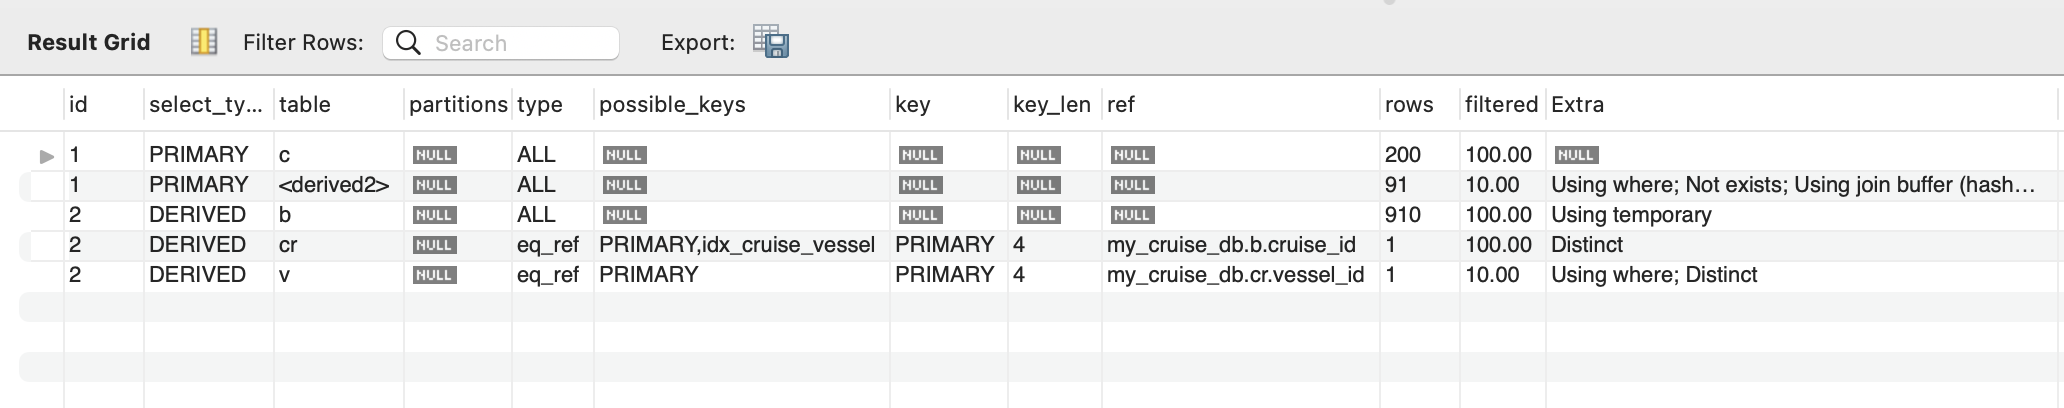
\includegraphics[width=\textwidth]{28.png} 
    \caption{Explain запроса 6}
\end{figure}

Выявляет клиентов, которые никогда не путешествовали на судне "Дух" \newline через подзапрос с NOT IN. Альтернатива NOT EXISTS была бы более эффективна для больших баз данных.

$$
\pi_{\text{c.client\_id}, \text{c.client\_full\_name}} \Bigg(
\beta_{\text{c}}(\text{Client}) \triangle \pi_{\text{b.client\_id}} \Bigg(
$$

$$
\sigma_{\text{v.vessel\_name} = \text{'Дух'}} \Bigg(
\beta_{\text{b}}(\text{ClientCruiseCabin}) \bowtie \beta_{\text{cr}}(\text{Cruise}) \bowtie \beta_{\text{v}}(\text{Vessel})
\Bigg)\Bigg)
$$
\\
\\
\subsection{Запрос 7}
Найти клиентов которые обращались в турагенства больше чем клиент А.
\begin{lstlisting}[style=sqlstyle, label=sql:query1]
SELECT
    c.client_id,
    c.client_full_name,
    COUNT(cta.tour_agency_id) AS number_of_agencies_contacted
FROM
    Client c
JOIN
    ClientTourAgency cta ON c.client_id = cta.client_id
GROUP BY
    c.client_id, c.client_full_name
HAVING
    COUNT(cta.tour_agency_id) > (
        SELECT
            COUNT(cta_specific.tour_agency_id)
        FROM
            Client cl_specific
        JOIN
            ClientTourAgency cta_specific ON cl_specific.client_id = cta_specific.client_id
        WHERE
            cl_specific.client_full_name = 'Николаев Марк Владимирович' 
        GROUP BY
            cl_specific.client_id 
    )
ORDER BY
    number_of_agencies_contacted DESC;
\end{lstlisting}
\begin{figure}[h!]
    \centering
    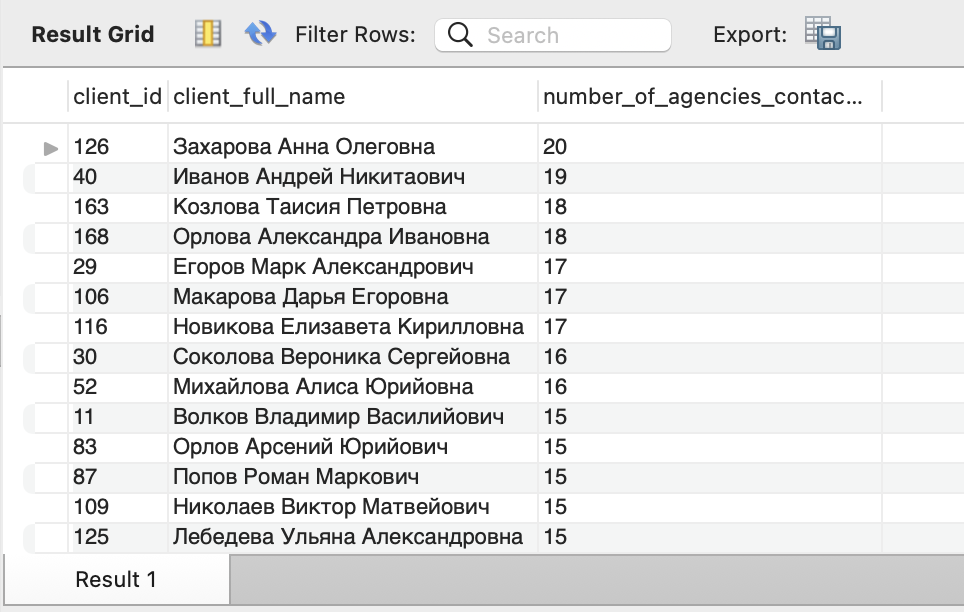
\includegraphics[width=0.7\textwidth]{24.png} 
    \caption{Результаты запроса 7}
\end{figure}
{\centering
Время выполнения запроса: 0:00:0.017.\par}
\begin{figure}[H]
    \centering
    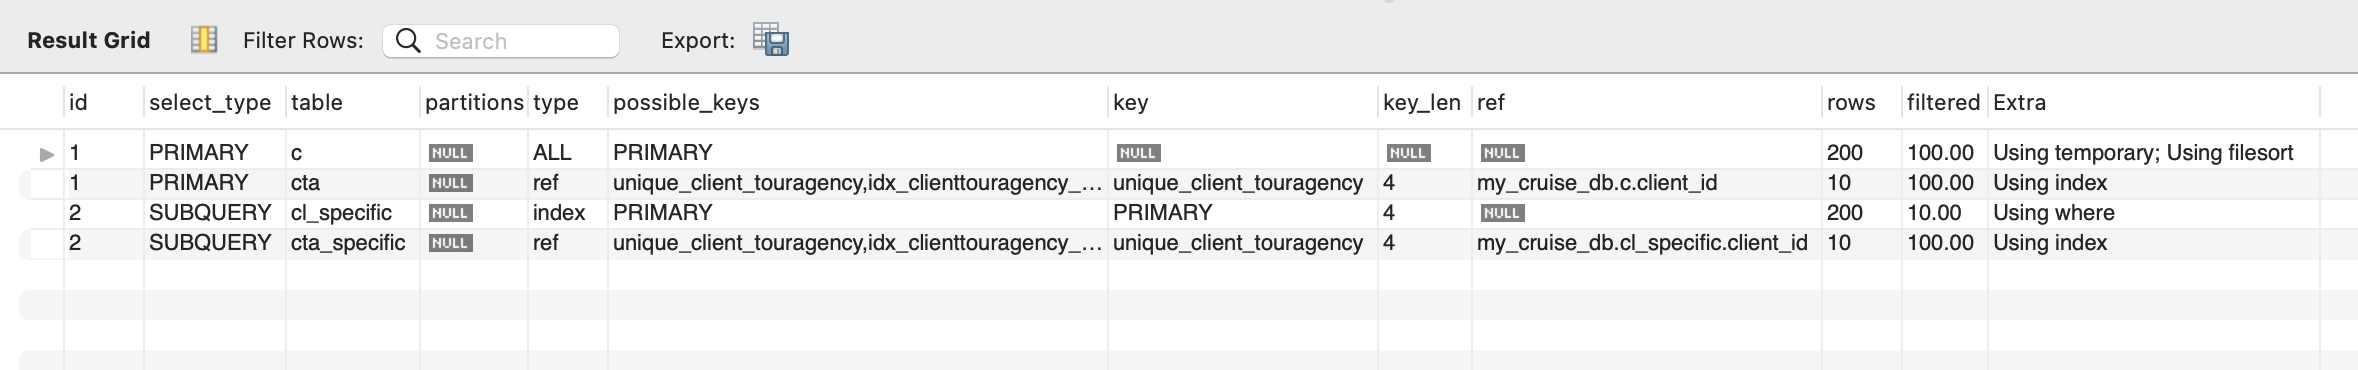
\includegraphics[width=\textwidth]{25.png} 
    \caption{Explain запроса 7}
\end{figure}

Находит клиентов, обращавшихся в большее число турагентств, чем Николаев М.В. Вложенный подзапрос вычисляет эталонное значение для сравнения в HAVING.

$$
\sigma_{\text{number\_of\_agencies\_contacted} > \text{count\_specific}} \Bigg(
\gamma_{\begin{subarray}{l}
\text{c.client\_id}, \\
\text{c.client\_full\_name}, \\
\text{COUNT(cta.tour\_agency\_id)}
\end{subarray}} \Bigg(
$$

$$
\beta_{\text{c}}(\text{Client}) \bowtie \beta_{\text{cta}}(\text{ClientTourAgency}) \Bigg)\Bigg)
$$


\subsection{Запрос 8}
Для каждого типа судна и типов кают посчитать число кают.
\begin{lstlisting}[style=sqlstyle, label=sql:query1]
SELECT
    vt.vessel_type_class AS тип_судна,
    ct.cabin_type_level AS тип_каюты,
    COUNT(cab.cabin_id) AS количество_кают
FROM
    VesselType vt
CROSS JOIN 
    CabinType ct
LEFT JOIN
    Vessel v ON vt.vessel_type_id = v.vessel_type_id 
LEFT JOIN
    Cabin cab ON v.vessel_id = cab.vessel_id AND cab.cabin_type_id = ct.cabin_type_id 
GROUP BY
    vt.vessel_type_class,
    ct.cabin_type_level
ORDER BY
    тип_судна,
    тип_каюты;
\end{lstlisting}
\begin{figure}[h!]
    \centering
    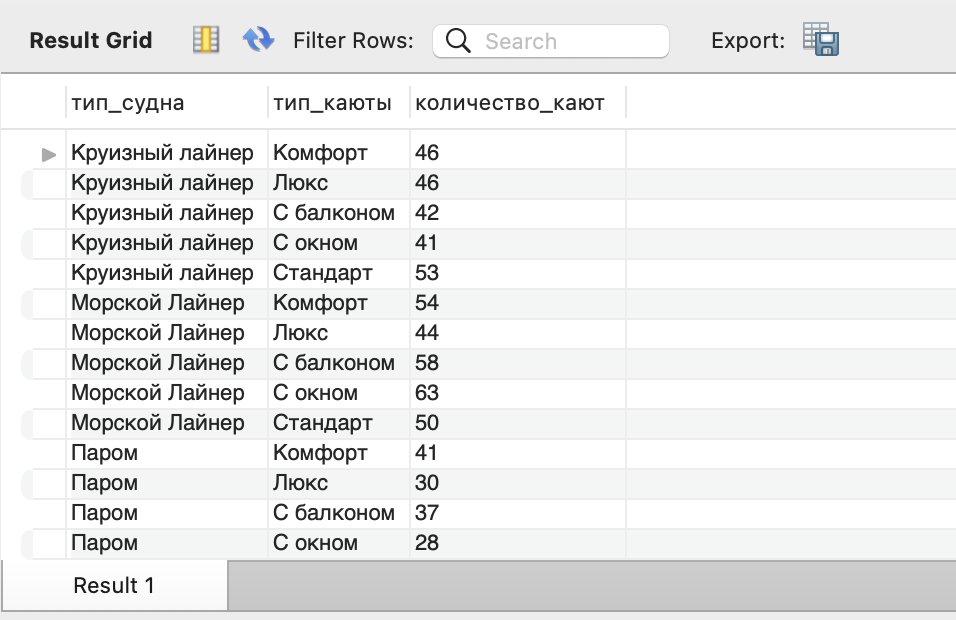
\includegraphics[width=0.7\textwidth]{26.png} 
    \caption{Результаты запроса 8}
\end{figure}
{\centering
Время выполнения запроса: 0:00:0.0011.\par}
\begin{figure}[H]
    \centering
    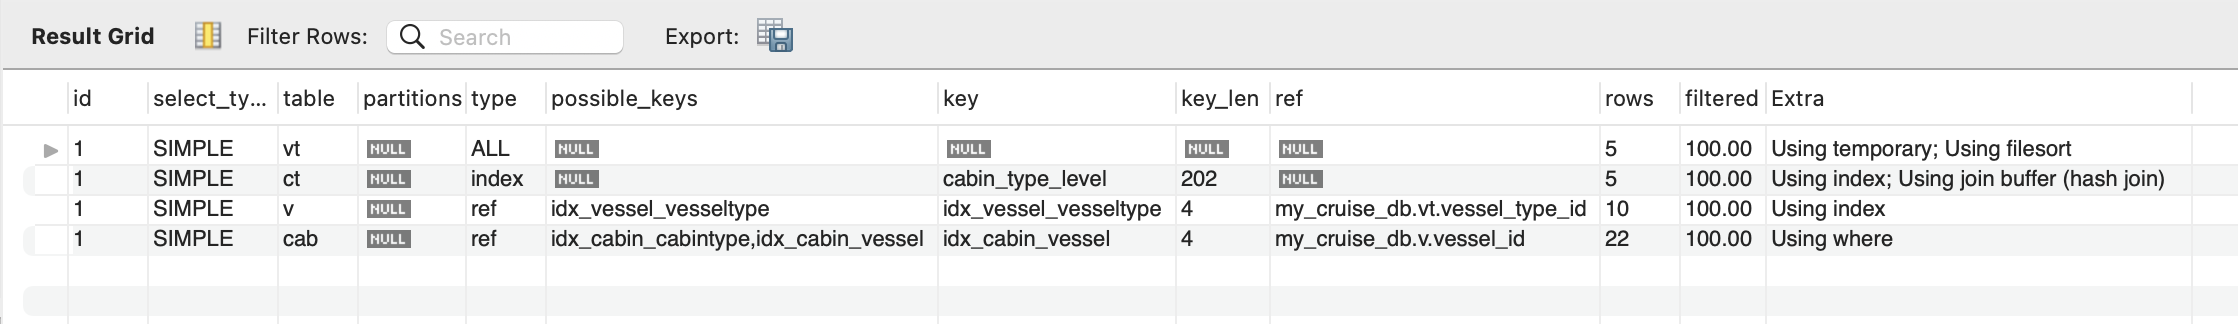
\includegraphics[width=\textwidth]{27.png} 
    \caption{Explain запроса 8}
\end{figure}

Создаёт матрицу "тип судна × тип каюты" с количеством кают в каждой ячейке. CROSS JOIN генерирует все возможные комбинации, а LEFT JOIN заполняет фактическими данными. Ниже представлены визуализация плана выполнения запроса (Рис.\ref{fig:expl8}) и 3D гистограмма (Рис.\ref{fig:hist8}).

$$
\gamma_{\begin{subarray}{l}
\text{vt.vessel\_type\_class}, \\
\text{ct.cabin\_type\_level}, \\
\text{COUNT(cab.cabin\_id)}
\end{subarray}} \Bigg(
$$

$$
\beta_{\text{vt}}(\text{VesselType}) \times \beta_{\text{ct}}(\text{CabinType}) \leftouterjoin \Big( \beta_{\text{v}}(\text{Vessel}) \bowtie \beta_{\text{cab}}(\text{Cabin}) \Big) \Bigg)
$$


\begin{figure}[H]
    \centering
    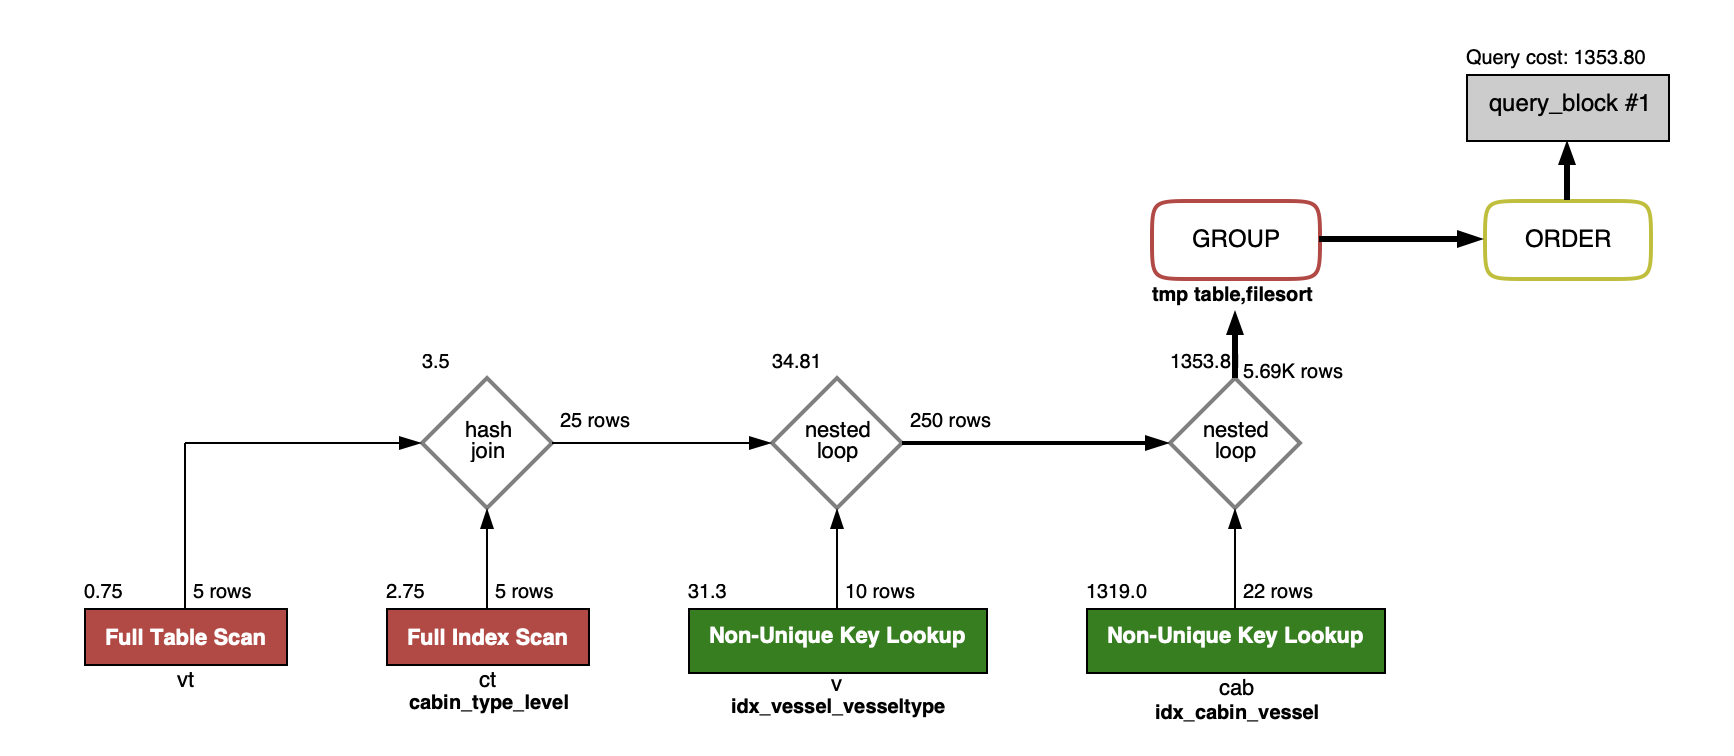
\includegraphics[width=\textwidth]{38.png} 
    \caption{Visual explain запроса 8}
    \label{fig:expl8}
\end{figure}

\begin{figure}[H]
    \centering
    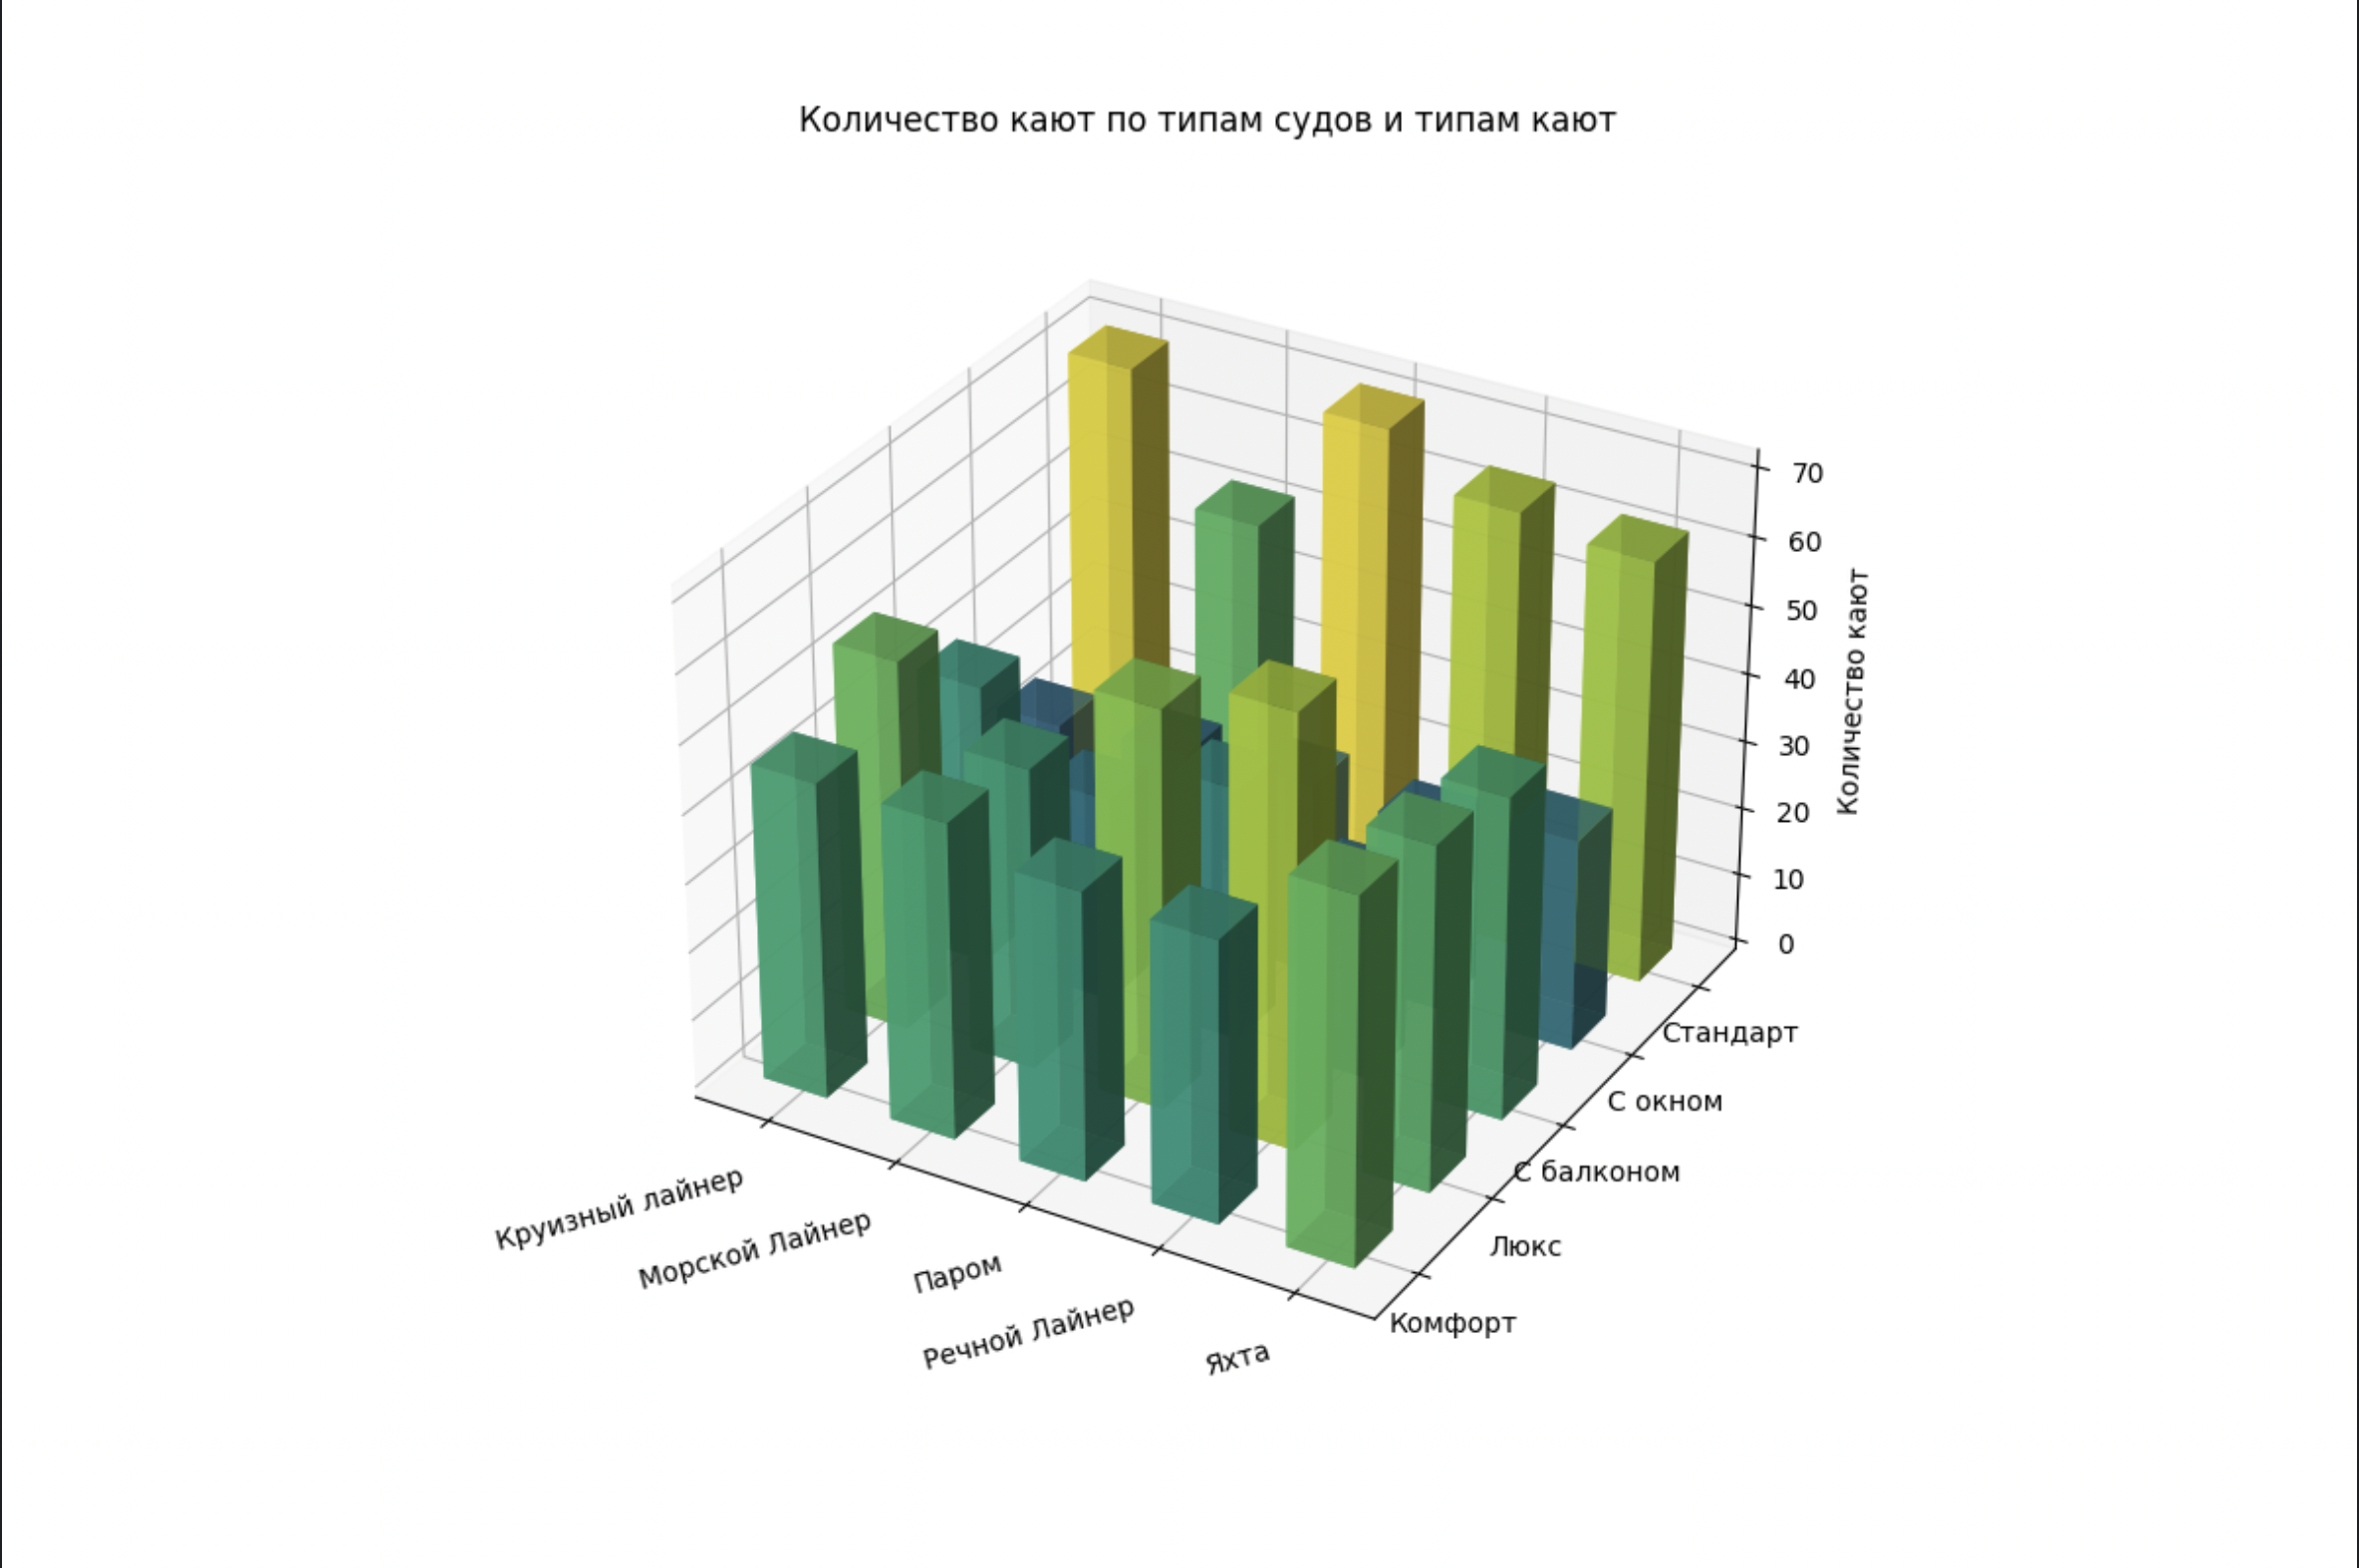
\includegraphics[width=\textwidth]{50.png} 
    \caption{3D гистограмма  запроса 8}
    \label{fig:hist8}
\end{figure}

\newpage
\section* {Заключение}
\addcontentsline{toc}{section}{Заключение}
\par В ходе работы был проведён анализ выбранной предметной об-
ласти, после чего были составлены ER-диаграмма, схема объектов базы дан-
ных и таблицы метаданных. На их основе, с учётом общих принципов проектирования систем управления базами данных \cite{sys}, были созданы таблицы в MySQL,
которые затем были заполнены с использованием программы на языке Python.
После этого было выполнено восемь запросов к базе данных, некоторые из
них представлены в 2 вариантах. Всего было создано 13 таблиц, в заполнен-
ной базе данных 254342 записей, на ER-диаграмме и схеме объектов базы
данных 9 сущностей.
\par Работа выполнялась на устройстве MacBook Pro с чипом Apple M1
и памятью 16ГБ, с использованием диалекта MySQL, среды программирова-
ния PyCharm, Python версии 3.8, командной строки и MySQL Workbench 8.0.31
Диаграммы результатов запросов были построены в PyCharm.


\newpage
\section* {Список использованных источников}
\addcontentsline{toc}{section}{Список использованных источников}
\begin{thebibliography}{9}
		
	\bibitem{sys}
	  Takahashi M., Azuma S., Trend C. L. The manga guide to databases. – No Starch Press, 2009. \\
	 \href {https://oberstar.eu.org/share/Documents/The-Manga-guide-to-databases.pdf}{https://oberstar.eu.org/share/Documents/The-Manga-guide-to-databases.pdf}

       \bibitem{Cruise.com}
	      Cruise.com - самый популярный сайт по водным круизам(последнее открытие 21.05.2025)\\	   
          \href{https://www.cruise.com}{https://www.cruise.com}	

    \bibitem{Royal}
	   Royal Caribbean Cruises - крупнейшая компания в мире и крупнейший держатель судов(последнее открытие 21.05.2025)\\	   
       \href{https://www.royalcaribbean.com}{https://www.royalcaribbean.com}	

    \bibitem{vodohod}
	   ВодоходЪ - лидер круизной отрасли в Росии(последнее открытие 21.05.2025)\\	   
       \href{https://vodohod.com/cruises/}{https://vodohod.com/cruises/}

    \bibitem{cruclub}
        Попов С. Г. Лекции по предмету «Теоретические основы баз данных». / Сергей Геннадьевич Попов. — СПбПУ, 2025. — Текст: электронный.(Дата обращения: 13.05.2025)
			
\end{thebibliography}

\newpage
\section* {Приложение А. Исходный код программы генерации схемы базы данных}
\addcontentsline{toc}{section}{Приложение А. Исходный код программы генерации схемы базы данных}
{\small 
\begin{verbatim}
import mysql.connector
import os

db_filename = 'my_cruise_database.db'
script_dir = os.path.dirname(__file__)
db_path = os.path.join(script_dir, db_filename)
print(f"Путь к файлу БД: {db_path}")
sql_schema_code = """
PRAGMA foreign_keys = ON; 

CREATE TABLE IF NOT EXISTS CabinType (
    cabin_type_id INTEGER PRIMARY KEY,
    cabin_type_level TEXT NOT NULL UNIQUE 
);

CREATE TABLE IF NOT EXISTS VesselType (
    vessel_type_id INTEGER PRIMARY KEY,
    vessel_type_class TEXT NOT NULL
);

CREATE TABLE IF NOT EXISTS CruiseType (
    cruise_type_id INTEGER PRIMARY KEY,
    cruise_type_name TEXT NOT NULL
);

CREATE TABLE IF NOT EXISTS СlientCruiseCabin (
    client_cruis_cabin_id INT AUTO_INCREMENT PRIMARY KEY,
    cruise_id INT NOT NULL,
    client_id INT NOT NULL,
    cabin_id INT NOT NULL
);

CREATE TABLE IF NOT EXISTS TravelAgency (
    agency_id INTEGER PRIMARY KEY,
    agency_name TEXT NOT NULL,
    vessel_id INTEGER NULL,
    client_id INTEGER NULL,
    cruise_id INTEGER NULL
);

CREATE TABLE IF NOT EXISTS TourOperator (
    tour_operator_id INTEGER PRIMARY KEY,
    agency_id INTEGER NULL,
    tour_operator_name TEXT NOT NULL,
    FOREIGN KEY (agency_id) REFERENCES TravelAgency(agency_id) 
    on delete no action 
    on update no action
);

CREATE TABLE IF NOT EXISTS TourAgency (
    tour_agency_id INTEGER PRIMARY KEY,
    tour_agency_name TEXT NOT NULL,
    agency_id INTEGER NULL,
    FOREIGN KEY (agency_id) REFERENCES TravelAgency(agency_id)
    on delete no action 
    on update no action
);

CREATE TABLE IF NOT EXISTS Client (
    client_id INTEGER PRIMARY KEY,
    client_full_name TEXT NOT NULL,
    client_history TEXT NULL,
    client_personal_data TEXT NULL,
    client_cabin_number TEXT NULL
);

CREATE TABLE IF NOT EXISTS Vessel (
    vessel_id INTEGER PRIMARY KEY,
    cabin_id INTEGER NULL, 
    vessel_capacity INTEGER NOT NULL,
    vessel_name TEXT NOT NULL,
    vessel_cabins_count INTEGER NOT NULL,
    agency_id INTEGER NULL,
    vessel_type_id INTEGER NOT NULL,
    FOREIGN KEY (agency_id) 
    REFERENCES TravelAgency(agency_id)
    on delete no action 
    on update no action,
    FOREIGN KEY (vessel_type_id) REFERENCES VesselType(vessel_type_id)
    on delete no action 
    on update no action
);

CREATE TABLE IF NOT EXISTS Cabin (
    cabin_id INTEGER PRIMARY KEY,
    cabin_type_id INTEGER NOT NULL,
    vessel_id INTEGER NOT NULL,
    FOREIGN KEY (cabin_type_id) 
    REFERENCES CabinType(cabin_type_id)
    on delete no action 
    on update no action,
    FOREIGN KEY (vessel_id) REFERENCES Vessel(vessel_id) 
    on delete no action on update no action
);

CREATE TABLE IF NOT EXISTS Cruise (
    cruise_id INTEGER PRIMARY KEY,
    cruise_type_id INTEGER NOT NULL,
    cruise_date TEXT NOT NULL, 
    cruise_name TEXT NOT NULL,
    vessel_id INTEGER NOT NULL,
    cruise_capacity INTEGER NULL,
    tour_operator_id INTEGER NOT NULL,
    FOREIGN KEY (cruise_type_id) 
    REFERENCES CruiseType(cruise_type_id)
    on delete no action 
    on update no action,
    FOREIGN KEY (vessel_id) REFERENCES Vessel(vessel_id) 
    on delete no action on update no action,
    FOREIGN KEY (tour_operator_id) REFERENCES
    TourOperator(tour_operator_id) on delete no action 
    on update no action
);

CREATE TABLE IF NOT EXISTS ClientTourAgency (
    client_tour_agency_id INTEGER PRIMARY KEY,
    client_id INTEGER NOT NULL,
    tour_agency_id INTEGER NOT NULL,
    FOREIGN KEY (client_id) REFERENCES Client(client_id) 
    on delete no action on update no action,
    FOREIGN KEY (tour_agency_id) 
    REFERENCES TourAgency(tour_agency_id)
    on delete no action 
    on update no action,
    UNIQUE (client_id, tour_agency_id)
);

CREATE TABLE IF NOT EXISTS CruiseTourAgency (
    cruise_tour_agency_id INTEGER PRIMARY KEY,
    cruise_id INTEGER NOT NULL,
    tour_agency_id INTEGER NOT NULL,
    FOREIGN KEY (cruise_id) REFERENCES Cruise(cruise_id) 
    on delete no action on update no action,
    FOREIGN KEY (tour_agency_id) 
    REFERENCES TourAgency(tour_agency_id)
    on delete no action 
    on update no action,
    UNIQUE (cruise_id, tour_agency_id)
);

"""
try:
    with mysql.connector.connect(db_path) as conn:
        cursor = conn.cursor()

        try:
            cursor.executescript(sql_schema_code)
            print("Схема БД успешно создана/обновлена.")
        except mysql.connector.Error as e:
            print(f"Ошибка при выполнении скрипта создания
            схемы: {e}")

        initial_cabin_types = [('Стандарт',), ('Люкс',),
        ('Премиум',)]
        try:
            cursor.executemany("INSERT OR IGNORE INTO CabinType
            (cabin_type_level) VALUES (?)", initial_cabin_types)
            print(f"Начальные данные в CabinType добавлены
            (или уже существовали). 
            Вставлено строк: {cursor.rowcount}")
        except mysql.connector.Error as e:
            print(f"Ошибка при вставке начальных данных в
            CabinType: {e}")

        try:
            cursor.execute("SELECT cabin_type_id, cabin_type_level 
            FROM CabinType")
            all_cabin_types = cursor.fetchall()
            print("\nТекущие типы кают в базе:")
            if not all_cabin_types:
                print("Таблица CabinType пуста.")
            else:
                for row in all_cabin_types:
                    print(row)
        except mysql.connector.Error as e:
            print(f"Ошибка при выборке данных из CabinType:
            {e}")

except mysql.connector.Error as e:
    print(f"Ошибка при подключении или работе с БД SQLite:
    {e}")

print("\nРабота с БД завершена.")
\end{verbatim}
}

\newpage
\section* {Приложение Б. Исходный код программы заполнения базы данных}
\addcontentsline{toc}{section}{Приложение Б. Исходный код программы заполнения базы данных}
{\small 
\begin{verbatim}
import mysql.connector
import random
import datetime

DB_CONFIG = {
    'host': 'localhost',
    'user': 'root',
    'password': '1a2s3d4f5g',
    'database': 'my_cruise_db'
}

NUM_TRAVEL_AGENCIES = 30
NUM_TOUR_AGENCIES = 80
MIN_OPERATORS_PER_AGENCY = 1
MAX_OPERATORS_PER_AGENCY = 6
NUM_CLIENTS = 200
MIN_CLIENTS_PER_TOUR_AGENCY = 20
MAX_CLIENTS_PER_TOUR_AGENCY = 30
NUM_VESSELS = 50
NUM_VESSEL_TYPES = 5
NUM_CRUISE_TYPES = 4
NUM_CABIN_TYPES = 5
MIN_CABINS_PER_VESSEL = 15
MAX_CABINS_PER_VESSEL = 30
NUM_CRUISES_PER_OPERATOR = 2200
MIN_TOUR_AGENCIES_PER_CRUISE = 60
MAX_TOUR_AGENCIES_PER_CRUISE = 80
СLIENT_CRUISE_CABIN_FILL_RATE = 0.80

def generate_random_date(start_days_offset=1, end_days_offset=365):
    """Генерирует случайную дату в будущем."""
    today = datetime.date.today()
    days_to_add = random.randint(start_days_offset, end_days_offset)
    return today + datetime.timedelta(days=days_to_add)

def batch_insert(cursor, query, data_list, batch_size=100):
    """Вставляет данные пакетами."""
    if not data_list:
        return
    for i in range(0, len(data_list), batch_size):
        batch = data_list[i:i + batch_size]
        try:
            cursor.executemany(query, batch)
        except mysql.connector.Error as err:
            print(f"Ошибка при пакетной вставке: {err}")
            print(f"Запрос: {query}")

def get_ids(cursor, table_name, id_column=None):
    """Получает список ID из таблицы."""
    if id_column is None:
        id_column = table_name.lower().replace(' ', '_') + '_id'
        if table_name.lower() == 'travelagency':
        id_column = 'agency_id'
        if table_name.lower() == 'touragency':
        id_column = 'tour_agency_id'
        if table_name.lower() == 'touroperator':
        id_column = 'tour_operator_id'

    try:
        cursor.execute(f"SELECT {id_column} FROM {table_name}")
        return [item[0] for item in cursor.fetchall()]
    except mysql.connector.Error as err:
        print(f"Ошибка при получении ID из таблицы
        {table_name}: {err}")
        return []

male_first_names = ["Александр", "Дмитрий", "Максим", "Сергей",
                    "Алексей", "Артем", "Илья", "Кирилл", "Михаил",
                    "Никита", "Матвей", "Роман", "Егор", "Арсений", 
                    "Иван", "Денис", "Евгений", "Тимофей",  
                    "Игорь", "Владимир", "Павел", "Руслан", "Марк", 
                    "Олег", "Юрий", "Виктор", "Василий", "Петр",
                    "Владислав", "Андрей"]
female_first_names = ["Анастасия", "Мария", "Анна", "Виктория",
                      "Елизавета", "Полина", "Алиса", "Дарья", 
                      "Александра", "Екатерина", "Ксения", "Арина",
                      "Вероника", "Василиса", "Варвара", "Милана", 
                      "Ева", "Ульяна", "Таисия", "Ольга", "Ирина",
                      "Светлана", "Наталья", "София", "Елена"]

last_names = ["Иванов", "Смирнов", "Кузнецов", "Попов", "Васильев",
              "Петров", "Соколов", "Михайлов", "Новиков",
              "Федоров", "Морозов", "Волков", "Алексеев", "Лебедев",
              "Семенов", "Егоров", "Павлов", "Козлов",
              "Степанов", "Николаев", "Орлов", "Андреев", "Макаров", 
              "Никитин", "Захаров", "Зайцев", "Соловьев",
              "Борисов", "Яковлев", "Григорьев"]

def generate_full_name():
    """Генерирует случайное ФИО."""
    gender = random.choice(['male', 'female'])

    if gender == 'male':
        first_name = random.choice(male_first_names)
        last_name = random.choice(last_names)
        patronymic_base = random.choice(male_first_names)
        patronymic = patronymic_base + "ович"
    else:
        first_name = random.choice(female_first_names)
        base_last_name = random.choice(last_names)
        if base_last_name.endswith("ов") 
        or base_last_name.endswith("ев")
        or base_last_name.endswith("ин"):
            last_name = base_last_name + "а"
        elif base_last_name.endswith("ий"):
            last_name = base_last_name[:-2] + "ая"
        else:
            last_name = base_last_name

        patronymic_base = random.choice(male_first_names)
        patronymic = patronymic_base + "овна"

    return f"{last_name} {first_name} {patronymic}"

cnx = None
cursor = None
try:
    print("Подключение к базе данных MySQL...")
    cnx = mysql.connector.connect(**DB_CONFIG)
    cursor = cnx.cursor()
    print("Подключение успешно.")

    print("Очистка существующих данных (если включено)...")
    cursor.execute("SET FOREIGN_KEY_CHECKS = 0;")
    tables_to_clear = [
        'ClientCruiseCabin', 'ClientTourAgency', 'CruiseTourAgency',
        'Cruise', 'Cabin', 'TourOperator',
        'Vessel', 'TourAgency',
        'TravelAgency', 'Client',
        'CabinType', 'VesselType', 'CruiseType'
    ]
    for table in tables_to_clear:
        try:
            print(f"  Очистка таблицы {table}...")
            cursor.execute(f"DELETE FROM {table}")
            cursor.execute(f"ALTER TABLE {table} AUTO_INCREMENT = 1")
        except mysql.connector.Error as err:
            print(f"Предупреждение: Не удалось очистить таблицу 
            {table} (возможно, ее нет): {err}")
    cursor.execute("SET FOREIGN_KEY_CHECKS = 1;")
    cnx.commit()
    print("Очистка завершена.")

    print("\n--- Генерация базовых типов ---")
    # 1. типы Кают (CabinType)
    cabin_types = [('Стандарт',), ('Комфорт',), ('С окном',), 
    ('С балконом',), ('Люкс',)]
    batch_insert(cursor, "INSERT INTO CabinType (cabin_type_level) 
    VALUES (%s)", cabin_types)
    print(f"Добавлено {len(cabin_types)} типов кают.")
    cabin_type_ids = get_ids(cursor, 'CabinType', 'cabin_type_id')

    # 2. типы Судна (VesselType)
    vessel_types = [('Яхта',), ('Речной Лайнер',), ('Паром',), 
    ('Морской Лайнер',), ('Круизный лайнер',)]
    batch_insert(cursor, "INSERT INTO VesselType (vessel_type_class)
    VALUES (%s)", vessel_types)
    print(f"Добавлено {len(vessel_types)} типов судов.")
    vessel_type_ids = get_ids(cursor, 'VesselType', 'vessel_type_id')

    # 3. типы Круиза (CruiseType)
    cruise_types = [('Речной',), ('Туристический',),
    ('Экскурсионный',), ('Тематический',)]
    batch_insert(cursor, "INSERT INTO CruiseType (cruise_type_name)
    VALUES (%s)", cruise_types)
    print(f"Добавлено {len(cruise_types)} типов круизов.")
    cruise_type_ids = get_ids(cursor, 'CruiseType', 'cruise_type_id')
    cnx.commit() # Применяем типы

    print("\n--- Генерация основных сущностей ---")
    # 4. клиенты (Client)
    clients_data = []
    for i in range(1, NUM_CLIENTS + 1):
        full_name = generate_full_name()
        history = random.choice(['Первый круиз', 'Постоянный клиент',
        None, 'Ездил в прошлом году'])
        passport = f"Паспорт {random.randint(1000, 9999)}
        {random.randint(100000, 999999)}"
        clients_data.append((full_name, history, passport))
    batch_insert(cursor, "INSERT INTO Client (client_full_name,
    client_history, client_personal_data) VALUES (%s, %s, %s)",
    clients_data)
    print(f"Добавлено {len(clients_data)} клиентов.")
    client_ids = get_ids(cursor, 'Client', 'client_id')
    cnx.commit()

    # 5. турфирмы (TravelAgency)
    agencies_data = [(f'Турфирма {i}',) for i in range(1,
    NUM_TRAVEL_AGENCIES + 1)]
    batch_insert(cursor, "INSERT INTO TravelAgency (agency_name)
    VALUES (%s)", agencies_data)
    print(f"Добавлено {len(agencies_data)} турфирм.")
    travel_agency_ids = get_ids(cursor, 'TravelAgency', 'agency_id')
    cnx.commit()

    # 6. турагентства (TourAgency)
    tour_agencies_data = []
    if travel_agency_ids:
        for i in range(1, NUM_TOUR_AGENCIES + 1):
            random_agency_id = random.choice(travel_agency_ids)
            tour_agencies_data.append((f'Турагентство {i}',
            random_agency_id))
        batch_insert(cursor, "INSERT INTO TourAgency
        (tour_agency_name, agency_id) VALUES (%s, %s)", 
        tour_agencies_data)
        print(f"Добавлено {len(tour_agencies_data)} турагентств.")
        tour_agency_ids = get_ids(cursor, 'TourAgency',
        'tour_agency_id')
    else:
        print("Нет турфирм (TravelAgency), пропускаем добавление
        турагентств.")
        tour_agency_ids = []
    cnx.commit()

    # 7. судна (Vessel)
    vessels_data = []
    vessels_cabins_info = {} # Словарь для хранения {vessel_id:
    cabins_count}
    if vessel_type_ids:
        vessel_name_parts = ["Мечта", "Звезда", "Надежда", "Орион",
                             "Жемчуг", "Лебедь", "Бриз", "Странник",
                             "Горизонт", "Компас", "Дельфин", 
                             "Королева", "Принцесса", "Императрица",
                             "Князь", "Адмирал", "Исследователь",
                             "Навигатор", "Путешественник", "Сияние",
                             "Ветер", "Гармония", "Песня", "Загадка",
                             "Дух", "Рассвет", "Нептун", "Посейдон",
                             "Танцор", "Магеллан"]
        for i in range(1, NUM_VESSELS + 1):
            name = f'"{random.choice(vessel_name_parts)}"'
            capacity = random.randint(50, 4000)
            cabins_count = random.randint(MIN_CABINS_PER_VESSEL,
            MAX_CABINS_PER_VESSEL)
            type_id = random.choice(vessel_type_ids)
            vessels_data.append((capacity, name, cabins_count
            , type_id))
        batch_insert(cursor, "INSERT INTO Vessel (vessel_capacity,
        vessel_name, vessel_cabins_count, vessel_type_id)
        VALUES (%s, %s, %s, %s)", vessels_data)
        print(f"Добавлено {len(vessels_data)} судов.")
        cursor.execute("SELECT vessel_id, vessel_cabins_count 
        FROM Vessel")
        vessels_cabins_info = dict(cursor.fetchall())
        vessel_ids = list(vessels_cabins_info.keys())
    else:
        print("Нет типов судов (VesselType), пропускаем 
        добавление судов.")
        vessel_ids = []
    cnx.commit()

    print("\n--- Генерация зависимых сущностей ---")

    # 8. туроператоры (TourOperator)
    operators_data = []
    if travel_agency_ids:
        for agency_id in travel_agency_ids:
            num_operators = random.randint(MIN_OPERATORS_PER_AGENCY,
            MAX_OPERATORS_PER_AGENCY)
            for i in range(1, num_operators + 1):
                operators_data.append((agency_id, f'Туроператор {i}
                для ТФ {agency_id}'))
        batch_insert(cursor, "INSERT INTO TourOperator (agency_id,
        tour_operator_name) VALUES (%s, %s)", operators_data)
        print(f"Добавлено {len(operators_data)} туроператоров.")
        tour_operator_ids = get_ids(cursor, 'TourOperator',
        'tour_operator_id')
    else:
        print("Нет турфирм (TravelAgency), пропускаем добавление
        туроператоров.")
        tour_operator_ids = []
    cnx.commit()

    # 9. каюты (Cabin)
    cabins_data = []
    cabins_by_vessel = {}
    if vessel_ids and cabin_type_ids:
        print("Генерация кают (может занять время)...")
        total_cabins_added = 0
        for vessel_id, cabins_count in vessels_cabins_info.items():
            vessel_cabins_list = []
            for _ in range(cabins_count):
                type_id = random.choice(cabin_type_ids)
                vessel_cabins_list.append((type_id, vessel_id))
            batch_insert(cursor, "INSERT INTO Cabin (cabin_type_id,
            vessel_id) VALUES (%s, %s)", vessel_cabins_list)
            total_cabins_added += len(vessel_cabins_list)
        print(f"Добавлено {total_cabins_added} кают.")
        cursor.execute("SELECT cabin_id, vessel_id FROM Cabin")
        all_cabins_raw = cursor.fetchall()
        for c_id, v_id in all_cabins_raw:
            if v_id not in cabins_by_vessel:
                cabins_by_vessel[v_id] = []
            cabins_by_vessel[v_id].append(c_id)
        print("Информация о каютах собрана.")
    else:
        print("Нет судов или типов кают, пропускаем 
        добавление кают.")
    cnx.commit()

    # 10. круизы (Cruise)
    cruises_data = []
    cruise_vessel_map = {}
    if cruise_type_ids and vessel_ids and tour_operator_ids:
        print("Генерация круизов (по 2000 на туроператора)...")
        cursor.execute("SELECT vessel_id, vessel_capacity 
        FROM Vessel")
        vessel_capacities = dict(cursor.fetchall())

        cruise_names_list = [
            "Летний Бриз", "Зимняя Сказка", "Золотая Осень", 
            "Весеннее Пробуждение", "Жемчужины Севера", 
            "Сокровища Южных Морей", "По Рекам Европы",
            "Арктическая Экспедиция", "Карибский Карнавал",
            "Средиземноморская Ривьера", "Волжские просторы",
            "Норвежские Фьорды", "Путешествие к Айсбергам",
            "Романтика Белых Ночей", "Острова Греции", 
            "Вино и Гастрономия", "Вокруг Света", 
            "Загадки Древних Цивилизаций", "Музыкальный Вояж",
            "Полярный Экспресс", "Звездный Путь", "Тропический Рай",
            "Тихоокеанская Легенда", "Очарование Востока", 
            "Историческое Наследие", "Круиз для Гурманов", 
            "В Поисках Приключений", "Семейные Каникулы",
            "Новогоднее Чудо", "Фото-тур по Фьордам"
        ]
        cruise_name_counter = 1

        for op_id in tour_operator_ids:
            for _ in range(NUM_CRUISES_PER_OPERATOR):
                if not cruise_type_ids or not vessel_ids:
                    print("Предупреждение: отсутствуют типы круизов
                    или суда, не могу создать круиз.")
                    continue

                type_id = random.choice(cruise_type_ids)
                v_id = random.choice(vessel_ids)
                date = generate_random_date()

                name = f'Круиз {cruise_name_counter} -
                {random.choice(cruise_names_list)} 
                (Оператор {op_id})'
                cruise_name_counter += 1

                capacity = vessel_capacities.get(v_id, 100)
                cruises_data.append((type_id, date, name, v_id, 
                capacity, op_id))

        batch_insert(cursor,
                     "INSERT INTO Cruise (cruise_type_id,
                     cruise_date, cruise_name, vessel_id,
                     cruise_capacity, tour_operator_id)
                     VALUES (%s, %s, %s, %s, %s, %s)",
                     cruises_data)
        print(f"Добавлено {len(cruises_data)} круизов.")
        cursor.execute("SELECT cruise_id, vessel_id FROM Cruise")
        cruise_vessel_map = dict(cursor.fetchall())
        cruise_ids = list(cruise_vessel_map.keys())
    else:
        print("Недостаточно данных (типы круизов/суда/туроператоры)
        для создания круизов.")
        cruise_ids = []
    cnx.commit()

    print("\n--- Генерация связующих таблиц ---")
    # 11. связь клиент-турагенство (ClientTourAgency)
    client_agency_links = []
    if client_ids and tour_agency_ids:
        print("Генерация связей Клиент-Турагенство...")
        for agency_id in tour_agency_ids:
            num_clients_for_agency = random.randint
            (MIN_CLIENTS_PER_TOUR_AGENCY,
            MAX_CLIENTS_PER_TOUR_AGENCY)
            if len(client_ids) > 0:
                selected_clients = random.sample(client_ids,
                min(num_clients_for_agency, len(client_ids)))
                for client_id in selected_clients:
                    client_agency_links.append((client_id,
                    agency_id))
        batch_insert(cursor, "INSERT IGNORE INTO ClientTourAgency 
        (client_id, tour_agency_id) VALUES (%s, %s)", 
        client_agency_links)
        print(f"Добавлено {len(client_agency_links)} связей 
        Клиент-Турагенство.")
    else:
        print("Нет клиентов или турагентств, пропускаем связи
        ClientTourAgency.")
    cnx.commit()

    # 12. связь круиз-турагенство (CruiseTourAgency)
    cruise_agency_links = []
    if cruise_ids and tour_agency_ids:
        print("Генерация связей Круиз-Турагенство (60-80 круизов
        на 1 турагентство)...")

        for agency_id in tour_agency_ids:
            num_cruises_for_agency = random.randint
            (MIN_TOUR_AGENCIES_PER_CRUISE, 
            MAX_TOUR_AGENCIES_PER_CRUISE)

            if not cruise_ids:  # Если список круизов пуст, нет
            смысла продолжать для этого агентства
                print(f"  Для турагентства ID {agency_id} нет
                доступных круизов для связи.")
                continue

            selected_cruises = random.sample(cruise_ids,
            min(num_cruises_for_agency, len(cruise_ids)))

            for cruise_id in selected_cruises:
                cruise_agency_links.append((cruise_id, agency_id))

        if cruise_agency_links:
            batch_insert(cursor, "INSERT IGNORE INTO CruiseTourAgency
            (cruise_id, tour_agency_id) VALUES (%s, %s)",
                         cruise_agency_links)
            print(
                f"  Добавлено (или попытались добавить)
                {len(cruise_agency_links)} связей Круиз-Турагенство.
                Успешно вставлено после IGNORE: {cursor.rowcount}")
        else:
            print(
                "  Не удалось сгенерировать данные для связей Круиз-
                Турагенство (возможно, нет круизов
                или турагентств).")

    else:
        print("Нет круизов или турагентств, пропускаем связи 
        CruiseTourAgency.")
    cnx.commit()

    # 13. бронирования (ClientCruiseCabin)
    client_cruise_cabins_data = []
    if cruise_ids and client_ids and cabins_by_vessel and
    cruise_vessel_map:
        print("Генерация бронирований (заполнение 80% 
        от всех кают)...")

        all_cabin_ids_for_total_count = []
        for v_id_key in cabins_by_vessel:
            all_cabin_ids_for_total_count.extend(cabins_by_vessel
            [v_id_key])

        if not all_cabin_ids_for_total_count:
            print("Нет доступных кают для создания бронирований.")
        else:
            num_total_cabins = len(all_cabin_ids_for_total_count)
            target_client_cruise_cabins = int(num_total_cabins *
            СLIENT_CRUISE_CABIN_FILL_RATE)
            print(
                f"  Всего кают: {num_total_cabins}, Целевое кол-во
                бронирований ({СLIENT_CRUISE_CABIN_FILL_RATE
                * 100}%):
                {target_client_cruise_cabins}")

            if target_client_cruise_cabins <= 0:
                print("  Целевое количество бронирований равно 0, 
                бронирования не создаются.")
            else:
                attempt_limit = target_client_cruise_cabins * 3
                generated_count = 0

                used_cruise_client_pairs = set()
                used_cruise_cabin_pairs = set()

                if not cruise_ids: print("  Нет ID круизов для 
                генерации бронирований!");
                if not client_ids: print("  Нет ID клиентов для 
                генерации бронирований!");

                if cruise_ids and client_ids:
                    for _ in range(attempt_limit):
                        if generated_count >= 
                        target_client_cruise_cabins:
                            break

                        random_cruise_id = random.choice(cruise_ids)
                        random_client_id = random.choice(client_ids)

                        vessel_id_for_this_cruise = 
                        cruise_vessel_map.get(random_cruise_id)

                        if not vessel_id_for_this_cruise:
                            continue

                        cabins_on_this_specific_vessel = 
                        cabins_by_vessel.get
                        (vessel_id_for_this_cruise, [])

                        if not cabins_on_this_specific_vessel:
                            continue

                        random_cabin_id = 
                        random.choice(cabins_on_this_specific_vessel)

                        if (random_cruise_id, random_client_id) 
                        not in used_cruise_client_pairs and \
                                (random_cruise_id, random_cabin_id) 
                                not in used_cruise_cabin_pairs:
                            client_cruise_cabins_data.append
                            ((random_cruise_id, random_client_id, 
                            random_cabin_id))
                            used_cruise_client_pairs.add
                            ((random_cruise_id, random_client_id))
                            used_cruise_cabin_pairs.add
                            ((random_cruise_id, random_cabin_id))
                            generated_count += 1
                else:
                    print("  Пропуск генерации бронирований из-за
                    отсутствия необходимых ID (круизы или клиенты).")

                if client_cruise_cabins_data:
                    batch_insert(cursor,
                                 "INSERT IGNORE INTO 
                                 ClientCruiseCabin
                                 (cruise_id, client_id, cabin_id) 
                                 VALUES (%s, %s, %s)",
                                 client_cruise_cabins_data)
                    print(
                        f"  Добавлено (или попытались добавить) 
                        {len(client_cruise_cabins_data)}
                        бронирований. Успешно вставлено
                        после IGNORE (приблизительно):
                        {cursor.rowcount}")
                else:
                    print("  Не удалось сгенерировать данные для бронирования.")
    else:
        print("Недостаточно данных (круизы/клиенты/каюты/
        связь_круиз_судно) для создания бронирований.")
    cnx.commit()

    print("\n--- Генерация данных завершена успешно! ---")

    print("\n--- Подсчет общего количества строк в базе данных ---")
    total_rows = 0
    tables_for_counting = [
        'CabinType', 'VesselType', 'CruiseType', 'Client', 'Cabin', 
        'TravelAgency', 'TourAgency', 'Vessel', 'TourOperator', 'Cruise',
        'ClientTourAgency', 'CruiseTourAgency', 'ClientCruiseCabin'
    ]

    if cnx and cnx.is_connected() and cursor:
        for table_name in tables_for_counting:
            try:
                cursor.execute(f"SELECT COUNT(*) FROM {table_name}")
                count = cursor.fetchone()[0]
                print(f"Количество строк в таблице 
                {table_name}: {count}")
                total_rows += count
            except mysql.connector.Error as err:
                print(f"Ошибка при подсчете строк в таблице 
                {table_name}: {err}")

        print(f"\nОБЩЕЕ КОЛИЧЕСТВО СТРОК ВО ВСЕХ УЧИТЫВАЕМЫХ
        ТАБЛИЦАХ:
        {total_rows}")
        if 250000 <= total_rows <= 350000:
            print("Общее количество строк находится в ожидаемом 
            диапазоне (250,000 - 350,000).")
        else:
            print("ВНИМАНИЕ: Общее количество строк НЕ находится
            в ожидаемом диапазоне (250,000 - 350,000).")

except mysql.connector.Error as err:
    print(f"Ошибка MySQL: {err}")
    if cnx and cnx.is_connected():
         print("Откатываем транзакцию...")
         cnx.rollback()
finally:
    if cursor:
        cursor.close()
        print("Курсор закрыт.")
    if cnx and cnx.is_connected():
        cnx.close()
        print("Соединение с MySQL закрыто.")
\end{verbatim}
}
\end{document}
